\documentclass[class=smolathesis,crop=false]{standalone}

\begin{document}

\chapter{Case Studies}
\label{ch:cases}

In this chapter we describe a number of case studies that demonstrate the main features of our framework in a variety of domains.

In Section~\ref{sec:cases/marking} we demonstrate the process transformations described in Section~\ref{sec:proc/transform} by modelling the process of marking a coursework assignment.
We start with an abstract model of the process, which we then refine to include knowledge about the students taking part in the coursework.
This refinement allows us to better capture the practical reality of the process.
The transformation functions automate the refinement, while their formal verification ensures they preserve validity of the abstract composition.

In Section~\ref{sec:cases/three-socks} we recreate an example used by Dixon et al.~\cite{dixon_et_al-2009} and demonstrate the use of non-deterministic resource combinations and our \isa{Anything} resource.
This domain concerns picking socks from a drawer until we have two of the same colour, for which we formalise two plans: one conformant and one contingent.

In Section~\ref{sec:cases/assembly} we model assembly workflows in the context of manufacturing metal components.
To effectively model the whole range of possible workflows, we define a recursive function that builds tailored process compositions from data available when the component is ordered.
We then prove that, for any possible order, the resulting process composition is valid.

In Section~\ref{sec:cases/factorio} we model manufacturing in the logistics simulation game Factorio\footnote{\url{https://factorio.com/}}.
We formalise the domain in such a way that valid process compositions represent manufacturing processes free from bottlenecks and with correct logistics connections.
We implement one such process in the game by following instructions derived from its formal description, and validate that the production rates and power usage match those computed in Isabelle/HOL.

\cbstart
Note that, while we implement most of the models in this chapter in Isabelle/HOL, one could also do so with code generated from our framework into Haskell (or, indeed, any other target language supported by the code generator).
The definitions would be nearly identical, because the necessary range of functions is extracted with the same names.
This is demonstrated by our formalisation of picking matching socks in Section~\ref{sec:cases/three-socks} which is done fully in Haskell.
What we lose by working outside the proof assistant is our ability to prove properties of these definitions, such as validity of the result for all possible parameters (as we do for instance for the assembly workflows in Lemma~\ref{isa:assembly/correct}).
In exchange we get improved performance and interoperability, since we no longer require that everything be formally verified.
\cbend

\section{Model of Coursework Marking}
\label{sec:cases/marking}

Recall our process transformations from Section~\ref{sec:proc/transform}.
They allow us to systematically transform and refine resources and processes, preserving a formal connection between the original and the result.
We now use the example domain of marking a coursework assignment to demonstrate how they can refine a process outline with additional information.

This domain concerns the lifetime of the coursework, from its release to the students, through their submission to eventually releasing marks back to the students.
Initially, we only know that the coursework will take place and the outline of the marking process.
Later, we obtain the specific students who will take part and can thus refine the outline.
Our process transformations allow us to take advantage of the new information without having to remake the process from scratch.

In our initial model, the resources moving between the relevant actions are quite abstract: for example, we represent all students as one resource atom.
As a result, that initial model is overly constrained compared to the process in practice: for example, it requires that all student submissions be marked before any mark can be submitted.
Once refined with information about the students taking part, this unwanted synchronisation can be removed.

We next introduce the initial model and then the concrete refinements that integrate information about the students taking part.
Note that our model could be made more complex to cover further aspects of coursework marking in practice, such as late submissions, non-submissions or internal dependencies within the coursework structure.
We use a simpler model to better demonstrate the transformations, but the same approach would apply to those extensions.

\subsection{Initial Model}
\label{sec:cases/marking/init}

We start our initial model with the resource atoms it involves.
The linear atoms cover: the students taking part, their submissions, their marks, the fact that the marks have been submitted and the fact that all marks have been released.
\begin{isadef}[Initial linear resource atoms]{isa:marking/lres}
  \isacomm{datatype}\ lres\ {\isacharequal}\ Students\ {\isacharbar}\ Submissions\ {\isacharbar}\ Marks\ {\isacharbar}\ MarksSubmitted\ {\isacharbar}\ MarksReleased

\end{isadef}

The single copyable atom we introduce represents the coursework instructions, such as a list of problems to solve.
Note that our initial model does not require it to be copyable, but in the refined model we will want to copy it for each student taking part.
\begin{isadef}[Copyable resource atoms]{isa:marking/cres}
  \isacomm{datatype}\ cres\ {\isacharequal}\ Instructions

\end{isadef}

Next, we define the primitive actions that the model will use.
These are the basic steps of the process: students making their submissions, marking the submissions, submitting the marks into the system and releasing those marks back to the students once they are all submitted.
We mechanise all of these as primitive actions with a simple string label and no metadata:
\begin{isadef}[Collecting submissions]{isa:marking/actions}
  \isacomm{definition}\ {\isachardoublequoteopen}collectSubs\ {\isacharequal}\isanewline
\ \ Primitive\ {\isacharparenleft}Copyable\ Instructions\ {\isasymodot}\ Res\ Students{\isacharparenright}\ {\isacharparenleft}Res\ Submissions{\isacharparenright}\isanewline
\isaindent{\ \ Primitive\ }\isaString{Collect\ Submissions}\ {\isacharparenleft}{\isacharparenright}{\isachardoublequoteclose}

\item
  \isacomm{definition}\ {\isachardoublequoteopen}markAll\ {\isacharequal}\isanewline
\ \ Primitive\ {\isacharparenleft}Res\ Submissions{\isacharparenright}\ {\isacharparenleft}Res\ Marks{\isacharparenright}\isanewline
\isaindent{\ \ Primitive\ }\isaString{Mark\ Submissions}\ {\isacharparenleft}{\isacharparenright}{\isachardoublequoteclose}

\item
  \isacomm{definition}\ {\isachardoublequoteopen}submitMarks\ {\isacharequal}\isanewline
\ \ Primitive\ {\isacharparenleft}Res\ Marks{\isacharparenright}\ {\isacharparenleft}Res\ MarksSubmitted{\isacharparenright}\isanewline
\isaindent{\ \ Primitive\ }\isaString{Submit\ Marks}\ {\isacharparenleft}{\isacharparenright}{\isachardoublequoteclose}

\item
  \isacomm{definition}\ {\isachardoublequoteopen}releaseMarks\ {\isacharequal}\isanewline
\ \ Primitive\ {\isacharparenleft}Res\ MarksSubmitted{\isacharparenright}\ {\isacharparenleft}Res\ MarksReleased{\isacharparenright}\isanewline
\isaindent{\ \ Primitive\ }\isaString{Release\ Marks}\ {\isacharparenleft}{\isacharparenright}{\isachardoublequoteclose}

\end{isadef}

The full process composition is simple in this initial model, all four actions are composed in sequence.
We visualise it with the process diagram in Figure~\ref{fig:marking-init}, and prove that it is valid and has the desired input and output:
\begin{isalemma}[Input, output and validity of the initial marking model]{isa:marking-before}
  \isacomm{lemma}\ marking{\isacharcolon}\isanewline
\ \ \isaOcomm{shows}\ \isapars{marking}:\ Copyable\ Instructions\ \isasymodot\ Res\ Students\ \isasymrightarrow\ Res\ MarksReleased\isanewline
\ \ \ \ \ \ \isaOcomm{and}\ valid\ marking\isanewline
\ \ \isacomm{by}\ \isapars{simp{\isacharunderscore}all\ \quasi{add{\isacharcolon}}\ markingProcess{\isacharunderscore}def\ action{\isacharunderscore}defs}

\end{isalemma}

Note how the monolithic resource atom and primitive actions impose constraints on the process that we may not want in practice.
For instance, we may want to mark submissions and submit the resulting marks in batches.
But for that we need to integrate more knowledge into the model.

\subsection{Refined Model}
\label{sec:cases/marking/ref}

The knowledge we integrate is that our initial abstraction of ``students'' actually consists of a number of individuals, producing individual submissions and requiring individual marks.
This then allows us to model that the individual marking actions do not depend on each other, which in turn allows their execution to interleave.
That better reflects the practical reality.

To model the new knowledge, we enclose the refined model in a locale that fixes a list of students (which we call \isa{students}) drawn from the type variable \isa{\isatv{s}}.
We name this locale \isa{refined} and enclose the initial model in a trivial locale called \isa{abstract} to avoid any name clashes.
In the \isa{refined} locale we also fix a function \isa{name} that assigns a string literal to every member of that type, representing the student's name for purposes of visualisation.
\begin{isadef}[Refinement locale with named students]{isa:marking/refined}
  \isacomm{locale}\isamarkupfalse%
\ refined\ {\isacharequal}\isanewline
\ \ \isaOcomm{fixes}\ \isafv{students}\ {\isacharcolon}{\isacharcolon}\ {\isachardoublequoteopen}\isatv{s}\ list{\isachardoublequoteclose}\ \isaOcomm{and}\ \isafv{name}\ {\isacharcolon}{\isacharcolon}\ {\isachardoublequoteopen}\isatv{s}\ {\isasymRightarrow}\ String{\isachardot}literal{\isachardoublequoteclose}

\end{isadef}

We make this refinement in two main steps: refinement of resources and refinement of actions.
As a target for the refinement of resources, we define a new datatype of linear resources to represent the more individual view (we keep the same copyable atom type \isa{cres}):
\pagebreak
\begin{isadef}[Elaborated linear resource atoms]{isa:marking/refined-lres}
  \isacomm{datatype}\ \isatv{s}\ lres\ {\isacharequal}\ Student\ \isapars{\isatv{s}}\ {\isacharbar}\ Submission\ \isapars{\isatv{s}}\ {\isacharbar}\ Mark\ \isapars{\isatv{s}}\isanewline
\isaindent{\isacomm{datatype}\ \isatv{s}\ lres\ }\widthtoL{\isacharbar}{\isacharequal}\ MarkSubmitted\ \isapars{\isatv{s}}\ {\isacharbar}\ MarksReleased

\end{isadef}

Then we can define the function that refines the linear atoms of the initial model into resources of the refined model.
For instance, the original atom \isa{Students} is mapped to a parallel combination of \isa{Student\ \isafv{s}} resources for \isa{\isafv{s}} from \isa{students}.
\begin{isadef}[Refining initial linear atoms into elaborated resources]{isa:refinement}
  \isacomm{primrec}\isamarkupfalse%
\ refinement\ {\isacharcolon}{\isacharcolon}\ {\isachardoublequoteopen}abstract{\isachardot}lres\ {\isasymRightarrow}\ \isapars{\isatv{s}\ refined{\isachardot}lres,\ abstract{\isachardot}cres}\ resource{\isachardoublequoteclose}\isanewline
\ \ \isaOcomm{where}\isanewline
\ \ \ \ {\isachardoublequoteopen}\isafv{refinement}\ abstract{\isachardot}Students\ {\isacharequal}\ Parallel\ {\isacharparenleft}map\ {\isacharparenleft}Res\ {\isasymcirc}\ refined{\isachardot}Student{\isacharparenright}\ \isafv{students}{\isacharparenright}{\isachardoublequoteclose}\isanewline
\ \ {\isacharbar}\ {\isachardoublequoteopen}\isafv{refinement}\ abstract{\isachardot}Submissions\ {\isacharequal}\isanewline
\ \ \ \ \ \ Parallel\ {\isacharparenleft}map\ {\isacharparenleft}Res\ {\isasymcirc}\ refined{\isachardot}Submission{\isacharparenright}\ \isafv{students}{\isacharparenright}{\isachardoublequoteclose}\isanewline
\ \ {\isacharbar}\ {\isachardoublequoteopen}\isafv{refinement}\ abstract{\isachardot}Marks\ {\isacharequal}\ Parallel\ {\isacharparenleft}map\ {\isacharparenleft}Res\ {\isasymcirc}\ refined{\isachardot}Mark{\isacharparenright}\ \isafv{students}{\isacharparenright}{\isachardoublequoteclose}\isanewline
\ \ {\isacharbar}\ {\isachardoublequoteopen}\isafv{refinement}\ abstract{\isachardot}MarksSubmitted\ {\isacharequal}\isanewline
\ \ \ \ \ \ Parallel\ {\isacharparenleft}map\ {\isacharparenleft}Res\ {\isasymcirc}\ refined{\isachardot}MarkSubmitted{\isacharparenright}\ \isafv{students}{\isacharparenright}{\isachardoublequoteclose}\isanewline
\ \ {\isacharbar}\ {\isachardoublequoteopen}\isafv{refinement}\ abstract{\isachardot}MarksReleased\ {\isacharequal}\ Res\ refined{\isachardot}MarksReleased{\isachardoublequoteclose}%

\end{isadef}

We can then apply this refinement function to resources throughout the original process composition with the following term:
\begin{isabelle}
\centering
  process{\isacharunderscore}refineRes\ refinement\ \isapars{{\isasymlambda}\isabv{x}.\ \isabv{x}}\ abstract{\isachardot}marking
\end{isabelle}
Instantiating the locale with four illustrative students, the resulting composition is visualised in Figure~\ref{fig:marking-res}.
Using to the properties of \isa{process{\isacharunderscore}refineRes}, we prove that the composition remains valid and its input and output are suitably refined.
\begin{isalemma}[Input, output and validity after refining resources]{isa:marking_refined_resources}
  \isacomm{lemma}\ marking{\isacharunderscore}refined{\isacharunderscore}resources{\isacharcolon}\isanewline
\ \ \isaOcomm{defines}\ \isafv{x}\ \isasymequiv\ process{\isacharunderscore}refineRes\ refinement\ id\ abstract{\isachardot}marking\isanewline
\ \ \ \ \isaOcomm{shows}\ \isapars{\isafv{x}}{\isacharcolon}\ Copyable\ Instructions\ \isasymodot\ Parallel\ {\isacharparenleft}map\ {\isacharparenleft}Res\ {\isasymcirc}\ Student{\isacharparenright}\ \isafv{students}{\isacharparenright}\isanewline
\isaindent{\ \ \ \ \isaOcomm{shows}\ \isacharparenleft}\isasymrightarrow\ Res\ MarksReleased\isanewline
\ \ \ \ \ \ \ \ \isaOcomm{and}\ valid\ \isafv{x}\isanewline
\ \ \isacomm{by}\ \isapars{simp{\isacharunderscore}all\ \quasi{add{\isacharcolon}}\ abstract{\isachardot}marking{\isacharunderscore}def\ abstract{\isachardot}action{\isacharunderscore}defs\ refine{\isacharunderscore}resource{\isacharunderscore}par}

\end{isalemma}

With resources refined, we can use primitive action substitution (see Section~\ref{sec:proc/transform/proc-subst}) to break up the monolithic collection of submissions, their marking and the submission of marks.
For each of those, the substitution requires two definitions: a predicate defining the actions to be replaced and a function generating their replacements.
In our case, the three predicates use the input and output of the primitive actions to single them out, while the three functions compose the relevant number of individualised actions in parallel as a replacement.
The collection replacement also needs to make sufficient copies of the \isa{Instructions} resource and interleave them with the individual student resources.
We illustrate the substitution on the most complex example, the collection of submissions.

The first part is the target action predicate, which we call \isa{collectionSplit{\isacharunderscore}cond}.
In this replacement we are looking for refined \isa{collectSubs} actions, so the predicate is defined as follows:
\begin{isadef}[Predicate targeting collection of submissions]{isa:collectionSplit_cond}
  \isacomm{definition}\ collectionSplit{\isacharunderscore}cond\ {\isacharcolon}{\isacharcolon}\ {\isachardoublequoteopen}\isapars{\isatv{s}\ refined{\isachardot}lres,\ abstract{\isachardot}cres}\ resource\isanewline
\isaindent{\isacomm{definition}\ collectionSplit{\isacharunderscore}cond\ }{\isasymRightarrow}\ \isapars{\isatv{s}\ refined{\isachardot}lres,\ abstract{\isachardot}cres}\ resource\isanewline
\isaindent{\isacomm{definition}\ collectionSplit{\isacharunderscore}cond\ }{\isasymRightarrow}\ String{\isachardot}literal\ {\isasymRightarrow}\ unit\ {\isasymRightarrow}\ bool{\isachardoublequoteclose}\isanewline
\ \ \isaOcomm{where}\ {\isachardoublequoteopen}\isafv{collectionSplit{\isacharunderscore}cond}\ \isabv{in\ out\ l\ m}\ {\isacharequal}\ {\isacharparenleft}\isanewline
\ \ \ \ \isabv{in}\ {\isacharequal}\ Copyable\ abstract.Instructions\ {\isasymodot}\isanewline
\isaindent{\ \ \ \ \isabv{in}\ {\isacharequal}\ }Parallel\ {\isacharparenleft}map\ {\isacharparenleft}Res\ {\isasymcirc}\ refined{\isachardot}Student{\isacharparenright}\ \isafv{students}{\isacharparenright}\ {\isasymand}\isanewline
\ \ \ \ \isabv{out}\ {\isacharequal}\ Parallel\ {\isacharparenleft}map\ {\isacharparenleft}Res\ {\isasymcirc}\ refined{\isachardot}Submission{\isacharparenright}\ \isafv{students}{\isacharparenright}{\isacharparenright}

\end{isadef}

The second part is the individualised action that will form the replacement, taking in a copy of the coursework instructions and the individual student, and producing the individual submission:
\begin{isadef}[Collecting individual submission]{isa:collectStudent}
  \isacomm{definition}\ collectStudent\ {\isacharcolon}{\isacharcolon}\ {\isachardoublequoteopen}\isatv{s}\isanewline
\isaindent{\isacomm{definition}\ collectStudent\ }{\isasymRightarrow}\ \isapars{\isatv{s}\ refined{\isachardot}lres,\ abstract{\isachardot}cres,\ String.literal,\ unit}\ process{\isachardoublequoteclose}\isanewline
\ \ \isaOcomm{where}\ {\isachardoublequoteopen}\isafv{collectStudent}\ \isabv{s}\ {\isacharequal}\isanewline
\ \ \ \ Primitive\ {\isacharparenleft}Copyable\ abstract.Instructions\ {\isasymodot}\ Res\ {\isacharparenleft}Student\ \isabv{s}{\isacharparenright}{\isacharparenright}\isanewline
\isaindent{\ \ \ \ Primitive\ }{\isacharparenleft}Res\ {\isacharparenleft}Submission\ \isabv{s}{\isacharparenright}{\isacharparenright}\isanewline
\isaindent{\ \ \ \ Primitive\ }{\isacharparenleft}\isaString{Collect\ submission\ of\ }\ {\isacharplus}\ name\ \isabv{s}{\isacharparenright}\ {\isacharparenleft}{\isacharparenright}{\isachardoublequoteclose}

\end{isadef}

Before we can construct the actual replacement compositions, we need to copy our one \isa{Instructions} atom enough times to have one for each student.
The input of the \isa{collectStudent} action also requires that we then interleave these copies with the individual student actions.
In order to achieve both of these, we define the following two functions to construct the relevant compositions of resource actions.

One is \isa{duplicateToN\ \isafv{n\ x}}, which uses the \isa{Duplicate} action to produce \isa{\isafv{n}} copies of the copyable atom \isa{\isafv{x}}.
We define it by recursion on the natural number \isa{\isafv{n}}:
\pagebreak
\begin{isadef}[Duplicating an atom into \isa{\isafv{n}} copies]{isa:duplicateToN}
  \isacomm{fun}\isamarkupfalse%
\ duplicateToN\ {\isacharcolon}{\isacharcolon}\ {\isachardoublequoteopen}nat\ {\isasymRightarrow}\ \isatv{b}\ {\isasymRightarrow}\ {\isacharparenleft}\isatv{a}{\isacharcomma}\ \isatv{b},\ \isatv{l}{\isacharcomma}\ \isatv{m}{\isacharparenright}\ process{\isachardoublequoteclose}\isanewline
\ \ \isaOcomm{where}\isanewline
\ \ \ \ {\isachardoublequoteopen}\isafv{duplicateToN}\ {\isacharparenleft}Suc\ {\isadigit{0}}{\isacharparenright}\ \isabv{x}\ {\isacharequal}\ Identity\ {\isacharparenleft}Copyable\ \isabv{x}{\isacharparenright}{\isachardoublequoteclose}\isanewline
\ \ {\isacharbar}\ {\isachardoublequoteopen}\isafv{duplicateToN}\ {\isacharparenleft}Suc\ \isabv{n}{\isacharparenright}\ \isabv{x}\ {\isacharequal}\ Seq\ \isapars{Duplicate\ \isabv{x}}\isanewline
\isaindent{\ \ {\isacharbar}\ {\isachardoublequoteopen}\isafv{duplicateToN}\ {\isacharparenleft}Suc\ \isabv{n}{\isacharparenright}\ \isabv{x}\ {\isacharequal}\ Seq\ }\isapars{Par\ \isapars{Identity\ {\isacharparenleft}Copyable\ \isabv{x}{\isacharparenright}}\ \isapars{\isafv{duplicateToN}\ \isabv{n\ r}}}{\isachardoublequoteclose}\isanewline
\ \ {\isacharbar}\ {\isachardoublequoteopen}\isafv{duplicateToN}\ {\isadigit{0}}\ \isabv{x}\ {\isacharequal}\ Erase\ \isabv{x}{\isachardoublequoteclose}

\end{isadef}

The other is \isa{swapInterleave\ \isafv{xs\ ys}}, which uses the \isa{Swap} action to take two lists of parallel resources and interleave them.
It does so by recursively swapping the first element of \isa{\isafv{ys}} with all but the first element of \isa{\isafv{xs}} until either runs out:
\begin{isadef}[Interleaving two lists of resources]{isa:swapInterleave}
  \isacomm{fun}\ swapInterleave\ {\isacharcolon}{\isacharcolon}\ {\isachardoublequoteopen}\isapars{\isatv{a},\ \isatv{b}}\ resource\ list\ {\isasymRightarrow}\ \isapars{\isatv{a},\ \isatv{b}}\ resource\ list\isanewline
\isaindent{\isacomm{fun}\ swapInterleave\ }{\isasymRightarrow}\ {\isacharparenleft}\isatv{a}{\isacharcomma}\ \isatv{b},\ \isatv{l}{\isacharcomma}\ \isatv{m}{\isacharparenright}\ process{\isachardoublequoteclose}\isanewline
\ \ \isaOcomm{where}\isanewline
\ \ \ \ {\isachardoublequoteopen}\isafv{swapInterleave}\ {\isacharparenleft}\isabv{x}\ {\isacharhash}\ \isabv{xs}{\isacharparenright}\ {\isacharparenleft}\isabv{y}\ {\isacharhash}\ \isabv{ys}{\isacharparenright}\ {\isacharequal}\isanewline
\ \ \ \ \ \ Seq\ \isapars{Par\ \isapars{Par\ \isapars{Identity\ \isabv{x}}\ \isapars{Swap\ {\isacharparenleft}Parallel\ \isabv{xs}{\isacharparenright}\ \isabv{y}}}\ \isapars{Identity\ {\isacharparenleft}Parallel\ \isabv{ys}{\isacharparenright}}}\isanewline
\isaindent{\ \ \ \ \ \ Seq\ }\isapars{Par\ \isapars{Identity\ {\isacharparenleft}\isabv{x}\ {\isasymodot}\ \isabv{y}{\isacharparenright}}\ \isapars{\isafv{swapInterleave}\ \isabv{xs}\ \isabv{ys}}}{\isachardoublequoteclose}\isanewline
\ \ {\isacharbar}\ {\isachardoublequoteopen}\isafv{swapInterleave}\ {\isacharbrackleft}{\isacharbrackright}\ \isabv{ys}\ {\isacharequal}\ Identity\ {\isacharparenleft}Parallel\ \isabv{ys}{\isacharparenright}{\isachardoublequoteclose}\isanewline
\ \ {\isacharbar}\ {\isachardoublequoteopen}\isafv{swapInterleave}\ \isabv{xs}\ {\isacharbrackleft}{\isacharbrackright}\ {\isacharequal}\ Identity\ {\isacharparenleft}Parallel\ \isabv{xs}{\isacharparenright}{\isachardoublequoteclose}

\end{isadef}

With these two functions, we can construct the replacement process composition for collecting submissions.
This composition in sequence: duplicates the \isa{Instructions} atom for each student, then interleaves the copies with the student atoms and finally performs \isa{collectStudent} in parallel for each student\footnote{Full definition of \isa{par{\isacharunderscore}process{\isacharunderscore}list} is given in Appendix~\ref{app:process-list}.}:
\begin{isadef}[Replacement for abstract collection of submissions]{isa:collectionSplit_func}
  \isacomm{definition}\ collectionSplit{\isacharunderscore}func\ {\isacharcolon}{\isacharcolon}\ {\isachardoublequoteopen}\isapars{\isatv{s}\ refined{\isachardot}lres,\ abstract{\isachardot}cres}\ resource\isanewline
\isaindent{\isacomm{definition}\ collectionSplit{\isacharunderscore}func\ }{\isasymRightarrow}\ \isapars{\isatv{s}\ refined{\isachardot}lres,\ abstract{\isachardot}cres}\ resource\isanewline
\isaindent{\isacomm{definition}\ collectionSplit{\isacharunderscore}func\ }{\isasymRightarrow}\ String{\isachardot}literal\ {\isasymRightarrow}\ unit\isanewline
\isaindent{\isacomm{definition}\ collectionSplit{\isacharunderscore}func\ }{\isasymRightarrow}\ \isapars{\isatv{s}\ refined{\isachardot}lres,\ abstract{\isachardot}cres,\ String.literal,\ unit}\ process{\isachardoublequoteclose}\isanewline
\ \ \isaOcomm{where}\ {\isachardoublequoteopen}\isafv{collectionSplit{\isacharunderscore}func}\ \isabv{in\ out\ l\ m}\ {\isacharequal}\isanewline
\ \ Seq\ \isapars{Seq\ \isapars{Par\ \isapars{duplicateToN\ {\isacharparenleft}length\ \isafv{students}{\isacharparenright}\ Instructions}\isanewline
\isaindent{\ \ Seq\ {\isacharparenleft}Seq\ {\isacharparenleft}Par\ }\isapars{Identity\ {\isacharparenleft}Parallel\ {\isacharparenleft}map\ {\isacharparenleft}Res\ {\isasymcirc}\ refined{\isachardot}Student{\isacharparenright}\ \isafv{students}{\isacharparenright}{\isacharparenright}}}\isanewline
\isaindent{\ \ Seq\ {\isacharparenleft}Seq\ }\isapars{swapInterleave\ {\isacharparenleft}replicate\ {\isacharparenleft}length\ \isafv{students}{\isacharparenright}\ {\isacharparenleft}Copyable\ Instructions{\isacharparenright}{\isacharparenright}\isanewline
\isaindent{\ \ Seq\ {\isacharparenleft}Seq\ {\isacharparenleft}swapInterleave\ }{\isacharparenleft}map\ {\isacharparenleft}Res\ {\isasymcirc}\ refined{\isachardot}Student{\isacharparenright}\ \isafv{students}{\isacharparenright}}}\isanewline
\isaindent{\ \ Seq\ }\isapars{par{\isacharunderscore}process{\isacharunderscore}list\ {\isacharparenleft}map\ collectStudent\ \isafv{students}{\isacharparenright}}{\isachardoublequoteclose}

\end{isadef}

\cbar{Using a simpler variant of this pattern we construct target predicates and replacement functions to refine the marking and mark submission actions.}
We can apply all three action refinements after the resource refinement with the following term:
\begin{center}
  \begin{minipage}{0.8\textwidth}
    \begin{isabelle}
      process{\isacharunderscore}subst\ submitSplit{\isacharunderscore}cond\ submitSplit{\isacharunderscore}func\isanewline
      \isapars{\ process{\isacharunderscore}subst\ markSplit{\isacharunderscore}cond\ markSplit{\isacharunderscore}func\isanewline
      \ \ \isapars{\ process{\isacharunderscore}subst\ collectionSplit{\isacharunderscore}cond\ collectionSplit{\isacharunderscore}func\isanewline
      \ \ \ \ \isapars{\ process{\isacharunderscore}refineRes\ refinement\ \isapars{{\isasymlambda}\isabv{x}.\ \isabv{x}}\ abstract{\isachardot}marking}}}
    \end{isabelle}
  \end{minipage}
\end{center}

Instantiating the locale with the same four illustrative students, the fully refined composition is visualised in Figure~\ref{fig:marking-fin}.
Using to the properties of \isa{process{\isacharunderscore}subst}, we prove that the composition still remains valid and its input and output are unchanged from the resource refinement for any arbitrary list of students.
\begin{isalemma}[Input, output and validity after refining actions]{isa:marking_refined_actions}
  \isacomm{lemma}\ marking{\isacharunderscore}refined{\isacharunderscore}actions{\isacharcolon}\isanewline
\ \ \isaOcomm{shows}\ \isapars{refined{\isachardot}marking}{\isacharcolon}\isanewline
\isaindent{\ \ \isaOcomm{shows}\ {\isacharparenleft}r}Copyable\ Instructions\ \isasymodot\ Parallel\ {\isacharparenleft}map\ {\isacharparenleft}Res\ {\isasymcirc}\ Student{\isacharparenright}\ \isafv{students}{\isacharparenright}\ \isasymrightarrow\isanewline
\isaindent{\ \ \isaOcomm{shows}\ {\isacharparenleft}r}Res\ MarksReleased\isanewline
\ \ \ \ \ \ \isaOcomm{and}\ valid\ refined{\isachardot}marking\isanewline
\ \ \isacomm{using}\ marking{\isacharunderscore}refined{\isacharunderscore}resources\ \isacomm{by}\ \isapars{simp{\isacharunderscore}all\ \quasi{add{\isacharcolon}}\ refined{\isachardot}marking{\isacharunderscore}def}

\end{isalemma}

As a result, we have a model that better reflects the marking process without unnecessary synchronisation.
We construct it via refinements of an initial outline, representing the integration of more knowledge.
Most notably, if we were to change the initial model then our refinements would automatically project that change into the refined model.
We see that as an invaluable feature for the maintenance of complex process models.

% Use e.g. pdfarranger to rotate the page for PDF viewers
\begin{sidewaysfigure}
  \centering
  \begin{subfigure}{\textwidth}
    \centering
    \includesvg[scale=0.5]{img-gen/before_marking.svg}
    \caption{Process diagram of the initial marking model}
    \label{fig:marking-init}
  \end{subfigure}
  \par\bigskip
  \begin{subfigure}{\textwidth}
    \centering
    \includesvg[scale=0.5]{img-gen/after_marking_1.svg}
    \caption{Process diagram of the marking process after resource refinement}
    \label{fig:marking-res}
  \end{subfigure}
  \par\bigskip
  \begin{subfigure}{\textwidth}
    \centering
    \includesvg[width=\textwidth]{img-gen/after_marking_4.svg}
    \caption{Process diagram of the marking process after all resource and action refinements}
    \label{fig:marking-fin}
  \end{subfigure}
\end{sidewaysfigure}

\subsection{Concluding Remarks}
\label{sec:cases/marking/conc}

We chose marking to demonstrate process refinement, because it is a simple case where some information about the process is only available at a later point in time but contributes significantly to the process model.

Moreover, marking is often done by multiple people who need to coordinate their work.
While we do not implement this at present, we envision a graphical checklist built on top of this model to support that coordination (see future work in Section~\ref{sec:conc/future}).
In this tool, both the course organiser and the individual markers would be able to see the status of all submissions, which would help them more effectively mark all of them.

As the complexity of the process increases, the coordination effort saved by such a tool would also increase.
This could, for instance, be the case for coursework assignments that are split into multiple parts, with different markers for different parts.
Note that such a split into parts could also be performed in our framework as another refinement of the process in Figure~\ref{fig:marking-fin}.

\section{Three Socks Problem}
\label{sec:cases/three-socks}

The three socks problem is an example by Dixon~et~al.~\cite{dixon_et_al-2009}, which we use to demonstrate our non-deterministic and \isa{Anything} resources (see Section~\ref{sec:res/terms}) and the \isa{Forget} resource action (see Section~\ref{sec:proc/type/res}).
While their work focuses on using deduction in ILL to construct a plan (or, a process), our framework focuses on representing the structure of process compositions.
As such, we do not replicate their work in automatically finding the composition but rather represent the two plans that they discuss.

\cbstart
We also take this opportunity to demonstrate how compositions can be built outside the proof assistant using the code generated from our mechanisation (see Section~\ref{sec:intro/itp/codegen}).
As such, we use Haskell to implement the resources and process compositions in this section.
Note how, apart from the keywords of the language itself and capitalisation changes, the approach remains largely the same as within Isabelle.
The main difference is that we cannot prove properties of the processes.
\cbend

The setting is a simple case of non-determinism in daily life.
To quote the authors:
\begin{displayquote}
  \itshape
  The problem is to get a pair of socks from the back of a chest.
  Because of the location of the socks, their colour cannot be seen until they are taken.
  The two-colour version of this problem is when there are only black and white socks.
\end{displayquote}

The domain of this problem has three kinds of socks as linear resource atoms: black, white and hidden.
\cbstart
We represent these with a simple datatype with three constructors, one for each kind of sock.
\begin{lstlisting}[label=lst:socks-res,caption=Linear atoms for picking socks (with abbreviations),basicstyle=\footnotesize\ttfamily,columns=flexible,breaklines=true]
data LRes = Hidden | Black | White
  deriving (Eq, Read, Show)

hidden = res Hidden
black = res Black
white = res White
\end{lstlisting}

We have one action available to us in this domain: pick a hidden sock from the drawer.
The output is a sock that is no longer hidden but either black or white.
\begin{lstlisting}[label=lst:socks-pick,caption=Primitive action for picking a sock,basicstyle=\footnotesize\ttfamily,columns=flexible,breaklines=true,showstringspaces=false]
pick :: Process LRes () String ()
pick = Primitive hidden (nonD black white) "Pick sock" ()
\end{lstlisting}

For convenience, before building compositions, we also define \lstinline[language=haskell]{#} as infix syntax for the resource product as we did \isa{\isasymodot} in Definition~\ref{isa:resource_par}.
\begin{lstlisting}[label=lst:socks-resource_par,caption=Infix syntax for resource product,basicstyle=\small\ttfamily,columns=flexible,breaklines=true]
(#) :: Resource a b -> Resource a b -> Resource a b
(#) = resource_par
\end{lstlisting}
\cbend

In the case with three socks, our goal is to compose a process \isa{\isafv{P}} with the following input and output:
\begin{isabelle}
\centering
  \isafv{P}:\ Res\ Hidden\ \isasymodot\ Res\ Hidden\ \isasymodot\ Res\ Hidden\\
  \isasymrightarrow\\
  NonD\ \isapars{Res\ Black\ \isasymodot\ Res\ Black\ \isasymodot\ Anything}\ \isapars{Res\ White\ \isasymodot\ Res\ White\ \isasymodot\ Anything}
\end{isabelle}

Dixon et al.\ use the ILL term $\top$ (\texttt{top} in their notation) in the goal sequent for their plan to ``allow solutions containing more socks than needed.''
This is because in ILL it is valid to derive $\top$ from any proposition (via the ${\top}_R$ rule, see Figure~\ref{fig:ill-rules}), in this case a proposition representing any number of arbitrarily coloured socks.
While nothing else can be done in ILL with this $\top$ proposition, it is perfectly suited to standing in for any configuration of extra socks.

Our resource counterpart to ILL's $\top$ is the \isa{Anything} resource, which represents the presence of some resources without any details of them.
The resource action \isa{Forget} is our counterpart to the ${\top}_R$ rule, accepting any resource as input and producing the \isa{Anything} resource.

A conformant plan for this problem, such as the one shown by Dixon et al.~(see Listing~\ref{lst:dixon}), represents an agent \cbar{that does not react to the colour of the picked sock.
This means that it always uses the \isa{pick} action to resolve all three socks (in any order), even though in some cases it already has a matching pair after resolving only two}.
Each possible outcome is then massaged into the same form as the goal output.

\cbstart
\begin{lstlisting}[label=lst:dixon,caption=Conformant plan shown by Dixon et al.,basicstyle=\footnotesize\ttfamily,columns=flexible,breaklines=true,mathescape=true]
case_or (pick h$_1$)
($\lambda$b$_1$. case_or (pick h$_2$)
  ($\lambda$b$_2$. case_or (pick h$_3$) ($\lambda$b$_3$. inl b$_1$$\otimes$b$_2$$\otimes$b$_3$) ($\lambda$w$_3$. inl b$_1$$\otimes$b$_2$$\otimes$w$_3$))
  ($\lambda$w$_2$. case_or (pick h$_3$) ($\lambda$b$_3$. inl b$_1$$\otimes$b$_3$$\otimes$w$_2$) ($\lambda$w$_3$. inr w$_2$$\otimes$w$_3$$\otimes$b$_1$)))
($\lambda$w$_1$. case_or (pick h$_2$)
  ($\lambda$b$_2$. case_or (pick h$_3$) ($\lambda$b$_3$. inl b$_2$$\otimes$b$_3$$\otimes$w$_1$) ($\lambda$w$_3$. inr w$_1$$\otimes$w$_3$$\otimes$b$_2$))
  ($\lambda$w$_2$. case_or (pick h$_3$) ($\lambda$b$_3$. inr w$_1$$\otimes$w$_2$$\otimes$b$_3$) ($\lambda$w$_3$. inr w$_1$$\otimes$w$_2$$\otimes$w$_3$)))
\end{lstlisting}

Our composition representing the same plan, shown in Listing~\ref{lst:conformant}, is significantly longer because it is fully explicit about how each case is massaged into the goal output.
Note that this composition also starts with three \lstinline{pick} actions in parallel.
This is followed by a composition of only resource actions to merge the three non-deterministic outputs.
Figure~\ref{fig:threeSocks-conformant} shows the process diagram generated by this composition.

\begin{lstlisting}[label=lst:conformant,caption=Conformant plan using our framework,basicstyle=\footnotesize\ttfamily,columns=flexible,breaklines=true]
conformantPlan :: Process LRes () String ()
conformantPlan = seq_process_list
  [ par_process_list [pick, pick, pick]
  , OptDistrIn (nonD black white # nonD black white) black white
  , Opt
      (seq_process_list
        [ Swap (nonD black white # nonD black white) black
        , OptDistrIn (black # nonD black white) black white
        , Opt
            (seq_process_list
              [ Par (Identity black) (Swap (nonD black white) black)
              , OptDistrIn (black # black) black white
              , Opt (innerNoSwap True black) (innerNoSwap True white)])
            (seq_process_list
              [ Par (Identity black) (Swap (nonD black white) white)
              , OptDistrIn (black # white) black white
              , Opt (innerSmallSwap True) (innerBigSwap False)])])
      (seq_process_list
        [ Swap (nonD black white # nonD black white) white
        , OptDistrIn (white # nonD black white) black white
        , Opt
            (seq_process_list
              [ Par (Identity white) (Swap (nonD black white) black)
              , OptDistrIn (white # black) black white
              , Opt (innerBigSwap True) (innerSmallSwap False)])
            (seq_process_list
              [ Par (Identity white) (Swap (nonD black white) white)
              , OptDistrIn (white # white) black white
              , Opt (innerNoSwap False black) (innerNoSwap False white)])])]
  where fInj isLeft = if isLeft then InjectL else InjectR
        picked isLeft  = if isLeft then black else white
        unpicked isLeft  = if isLeft then white else black
        innerNoSwap isLeft r =
          let s = picked isLeft; f = fInj isLeft
          in Seq
              (Par (Identity (s # s)) (Forget r))
              (f (black # black # anything) (white # white # anything))
        innerSmallSwap isLeft =
          let s = picked isLeft; r = unpicked isLeft
          in Seq (Par (Identity s) (Swap r s)) (innerNoSwap isLeft r)
        innerBigSwap isLeft =
          let s = picked isLeft; r = unpicked isLeft
          in Seq (Swap r (s # s)) (innerNoSwap isLeft r)
\end{lstlisting}

In contrast, a contingent plan (not shown explicitly by Dixon et al.) represents an agent capable of reacting to the colour of the picked sock.
For instance, if the plan is being executed by a human, they could be looking at the socks as they pick them and stop once they have two of the same colour.
Same as with the conformant plan, the outcome in each case is massaged into the same form as the goal output, but in two cases the extra sock remains hidden.
The composition representing this plan is given in Listing~\ref{lst:contingent} in the Appendix and visualised in Figure~\ref{fig:threeSocks-contingent}.
\cbend

% Use e.g. pdfarranger to rotate both pages for PDF viewers
\begin{sidewaysfigure}
  \centering
  \includesvg[scale=0.45]{img-gen/threeSocks_conformant.svg}
  \caption{Process diagram of the conformant plan for picking two socks of the same colour}
  \label{fig:threeSocks-conformant}
\end{sidewaysfigure}
\begin{sidewaysfigure}
  \centering
  \includesvg[scale=0.45]{img-gen/threeSocks_contingent.svg}
  \caption{Process diagram of the contingent plan for picking two socks of the same colour}
  \label{fig:threeSocks-contingent}
\end{sidewaysfigure}

Compared to the term that Dixon et al.\ show for their conformant plan (Listing~\ref{lst:dixon}), our process composition is more explicit with respect to \emph{how} the outcomes are massaged to fit the goal output.
One part of this is that our composition framework is explicit about the order of parallel resources, which helps us avoid ambiguity.
This means that when we encounter \isa{Res\ Black\ \isasymodot\ Res\ White\ \isasymodot\ Res\ Black} we must use a swap action to match the first case of the goal output.
In the work of Dixon et al., this step does not explicitly appear in the resulting term.

Another point where our representation is more explicit is that we use the \isa{Forget} action to turn extra socks into the \isa{Anything} resource, while no equivalent step appears in the term shown by Dixon et al.
The connection between any remaining socks and the \texttt{top} term is made by the deduction that generates their plan.

This highlights a subtle difference in our two approaches: we are verifying that a process representing the plan has a certain output, while Dixon et al.\ are using proof search to generate a plan that satisfies their specification.
The conformant plan they present considers the expected eight outcomes resulting from three binary variables and it is in showing that it satisfies the specification that those outcomes are collapsed into two options.
In our case, we are deriving the precise output of the process and, as such, take explicit actions as part of that process to bring the outcomes into alignment.
This increased focus on the precise output stems from our interest in composition of processes, where their inputs and outputs feature prominently.

\section{Assembly Workflow Model}
\label{sec:cases/assembly}

As part of our previous work on WorkflowFM (see Section~\ref{sec:intro/pap/wfm}), we presented two case studies of formal manufacturing process models and their use to improve accuracy of scheduling production flows~\cite{papapa_et_al-2021}.
Those case studies focused on two kinds of process models: standard operating workflows and assembly workflows.
In this section we revisit the latter using our framework.

The advantage that our framework offers for assembly workflow is the ability to define compositions through recursive functions.
This allows us to generate compositions customised to every individual assembly, something that is not possible to model with compositions in WorkflowFM.
Crucially, we prove in general that every instance for any assembly order will be a valid composition.

\subsection{Assemblies}
\label{sec:cases/assembly/context}

The context for this case study is the manufacturing of metal components, with each job having a custom production flow.
As such, we organise the jobs into \emph{assemblies} that collect the required materials and perform a sequence of operations on them.
Crucially, each of the objects brought together can be another assembly, and, as a result, they form trees.
We call the data describing the assembly to be produced the \emph{assembly order}.

We wish to model the process of fulfilling an assembly order as the following steps:
\begin{enumerate}
  \item Fulfil all subassemblies,
  \item Gather all subassemblies and materials into one production lot,
  \item Perform each operation in sequence on the combined production lot.
\end{enumerate}

The high variability of assembly orders is what makes modelling this process difficult.
For instance, there is no limit on the breadth or depth of the assembly tree and so every model may have an arbitrary number of ``assemble'' actions and operation sequences.
Similarly, there is no limit to the number of operations in the sequence and so every model may have an arbitrary number of ``perform operation'' actions.
The precise values for these parameters are only known with a concrete assembly order, not at modelling time.

In the WorkflowFM model~\cite{papapa_et_al-2021}, this is handled outside of the reasoner as part of the simulation environment.
Using our present framework, we define a function from assembly orders to process compositions.
One could view this function as a kind of generic description of the process and the result of running the function for a particular order as the actual model.
This allows us to prove that these compositions are valid for all assembly orders.

\subsection{Assembly Order Formalisation}
\label{sec:cases/assembly/formal-order}

We start by formalising the assembly orders, which consist of other orders and operations.
In our model we give each order a string identifier and we label each operation with a string describing it.
In a practical setting these types could contain additional information, such as machine descriptions and configuration, possibly drawn from an enterprise resource planning (ERP) system.
\begin{isadef}[Datatypes for operations and assembly orders]{isa:assembly/order}
  \isacomm{datatype}\ operation\ \isacharequal\ Op\ \isapars{\isafv{op{\isacharunderscore}label}\isacharcolon\ String{\isachardot}literal}

\item
  \isacomm{datatype}\ order\ \isacharequal\isanewline
\ \ Order\ \isapars{\isafv{orderID}\isacharcolon\ String{\isachardot}literal}\ \isapars{\isafv{suborders}\isacharcolon\ order\ list}\ \isapars{\isafv{operations}\isacharcolon\ operation\ list}

\end{isadef}

\subsection{Resource Atoms}
\label{sec:cases/assembly/res}

The first part formalising this domain is the resource atoms.
Here all our atoms are linear: production lots (abstracting what in practice would be an identifier from an ERP system) and machines.
\begin{isadef}[Linear resource atoms]{isa:assembly/res}
  \isacomm{datatype}\ lres\ \isacharequal\ Lot\ \isacharbar\ Machine

\end{isadef}

We use string literals as labels for actions and attach no metadata to them.
Thus the process type for this domain is the following:
\begin{isabelle}
\centering
  \isapars{lres,\ unit,\ String.literal,\ unit}\ process
\end{isabelle}

\subsection{Primitive Actions}
\label{sec:cases/assembly/primitive}

The second part of formalising this domain is the primitive actions:
\begin{itemize}
  \item Reserve and free a machine.
    These represent interaction with the larger (unmodelled) environment of the factory and are a crucial point when simulating a large number of process instances from this domain with some shared pool of machines.
    In simulation, the implementation of reserving a machine would block until a machine was provided to it by the external environment.
    Note that by introducing this primitive we are making an assumption that it is always possible to eventually provide the machine.
    \begin{isadef}[Reserving and freeing a machine]{isa:assembly/actions-reserve}
      \isacomm{definition}\ {\isachardoublequoteopen}reserve\ {\isacharequal}\ Primitive\ Empty\ {\isacharparenleft}Res\ Machine{\isacharparenright}\ \isaString{Reserve\ machine}\ {\isacharparenleft}{\isacharparenright}{\isachardoublequoteclose}

    \item
      \isacomm{definition}\ {\isachardoublequoteopen}free\ {\isacharequal}\ Primitive\ {\isacharparenleft}Res\ Machine{\isacharparenright}\ Empty\ \isaString{Free\ machine}\ {\isacharparenleft}{\isacharparenright}{\isachardoublequoteclose}

    \end{isadef}
  \item Perform some operation using a machine on a production lot.
    \begin{isadef}[Performing an operation]{isa:assembly/actions-perform}
      \isacomm{definition}\ {\isachardoublequoteopen}perform\ \isafv{op}\ {\isacharequal}\isanewline
\ \ Primitive\ \isapars{Res\ Machine\ \isasymodot\ Res\ Lot}\ {\isacharparenleft}Res\ Machine\ \isasymodot\ Res\ Lot{\isacharparenright}\isanewline
\isaindent{\ \ Primitive\ }\isapars{\isaString{Do\ }\ {\isacharplus}\ op{\isacharunderscore}label\ \isafv{op}}\ {\isacharparenleft}{\isacharparenright}{\isachardoublequoteclose}

    \end{isadef}
  \item Bring a number of production lots together, each resulting from a subassembly.
    This also represents retrieving any required raw resources from storage.\footnotemark
    \begin{isadef}[Assembling lots for an order into one]{isa:assembly/actions-assemble}
      \isacomm{definition}\ {\isachardoublequoteopen}assemble\ \isafv{o}\ {\isacharequal}\isanewline
\ \ Primitive\ \isapars{Parallel\ \isapars{replicate\ \isapars{length\ \isapars{suborders\ \isafv{o}}}\ \isapars{Res\ Lot}}}\ {\isacharparenleft}Res\ Lot{\isacharparenright}\isanewline
\isaindent{\ \ Primitive\ }\isapars{\isaString{Assemble\ }\ {\isacharplus}\ orderID\ \isafv{o}}\ {\isacharparenleft}{\isacharparenright}{\isachardoublequoteclose}

    \end{isadef}
\end{itemize}

\footnotetext{
  We could also model this by expanding the assembly order type and adding another primitive action.
  This would complicate the model without enhancing our point, so we choose to keep our model simple for this discussion.
}

Note that interaction with the environment through the \isa{Reserve} action could lead to deadlock of multiple interacting process instances.
For instance, if there are two machines in the shared pool and two process instances each hold one and require reserving a second machine before they free the first one.
Modelling individual processes does not prevent this situation, we would have to model all of the interacting processes to guarantee deadlock freedom.

\subsection{Assembly Composition}
\label{sec:cases/assembly/comp}

First, recall that our goal process needs to perform a sequence of operations.
We define two functions, one that handles performing the operation while reserving and freeing a machine, and another to do this for a sequence of operations:
\begin{isadef}[Performing an operation with a machine\footnote{Full definition of \isa{seq{\isacharunderscore}process{\isacharunderscore}list} is given in Appendix~\ref{app:process-list}.}]{isa:assembly/op}
  \isacomm{fun}\isamarkupfalse%
\ op\ {\isacharcolon}{\isacharcolon}\ {\isachardoublequoteopen}operation\ {\isasymRightarrow}\ {\isacharparenleft}lres{\isacharcomma}\ String{\isachardot}literal{\isacharcomma}\ meta{\isacharparenright}\ process{\isachardoublequoteclose}\isanewline
\ \ \isaOcomm{where}\ {\isachardoublequoteopen}\isafv{op}\ \isabv{x}\ {\isacharequal}\ seq{\isacharunderscore}process{\isacharunderscore}list\ \isacharbrackleft\isanewline
\ \ \ \ Par\ reserve\ {\isacharparenleft}Identity\ {\isacharparenleft}Res\ Lot{\isacharparenright}{\isacharparenright}\isanewline
\ \ {\isacharcomma}\ perform\ \isabv{x}\isanewline
\ \ {\isacharcomma}\ Par\ free\ {\isacharparenleft}Identity\ {\isacharparenleft}Res\ Lot{\isacharparenright}{\isacharparenright}{\isacharbrackright}{\isachardoublequoteclose}

\end{isadef}
\begin{isadef}[Performing a sequence of operations]{isa:assembly/ops}
  \isacomm{fun}\isamarkupfalse%
\ ops\ {\isacharcolon}{\isacharcolon}\ {\isachardoublequoteopen}operation\ list\ {\isasymRightarrow}\ {\isacharparenleft}lres{\isacharcomma}\ String{\isachardot}literal{\isacharcomma}\ meta{\isacharparenright}\ process{\isachardoublequoteclose}\isanewline
\ \ \isaOcomm{where}\isanewline
\ \ \ \ {\isachardoublequoteopen}\isafv{ops}\ {\isacharbrackleft}{\isacharbrackright}\ {\isacharequal}\ Identity\ {\isacharparenleft}Res\ Lot{\isacharparenright}{\isachardoublequoteclose}\isanewline
\ \ {\isacharbar}\ {\isachardoublequoteopen}\isafv{ops}\ {\isacharbrackleft}\isabv{x}{\isacharbrackright}\ {\isacharequal}\ op\ \isabv{x}\isanewline
\ \ {\isacharbar}\ {\isachardoublequoteopen}\isafv{ops}\ {\isacharparenleft}\isabv{x}{\isacharhash}\isabv{xs}{\isacharparenright}\ {\isacharequal}\ Seq\ {\isacharparenleft}op\ \isabv{x}{\isacharparenright}\ {\isacharparenleft}ops\ \isabv{xs}{\isacharparenright}{\isachardoublequoteclose}

\end{isadef}

Next, the assembly process composition for any order is given in Definition~\ref{isa:assembly/assm}.
While defined using general recursion, it terminates because every suborder is necessarily smaller than the order that contains it.
\begin{isadef}[Assembling according to given order\footnote{Full definition of \isa{par{\isacharunderscore}process{\isacharunderscore}list} is given in Appendix~\ref{app:process-list}.}]{isa:assembly/assm}
  \isacomm{function}\isamarkupfalse%
\ assm\ {\isacharcolon}{\isacharcolon}\ {\isachardoublequoteopen}order\ {\isasymRightarrow}\ {\isacharparenleft}lres{\isacharcomma}\ String{\isachardot}literal{\isacharcomma}\ meta{\isacharparenright}\ process{\isachardoublequoteclose}\isanewline
\ \ \isaOcomm{where}\ {\isachardoublequoteopen}\isafv{assm}\ \isabv{x}\ {\isacharequal}\ seq{\isacharunderscore}process{\isacharunderscore}list\ \isacharbrackleft\isanewline
\ \ \ \ par{\isacharunderscore}process{\isacharunderscore}list\ {\isacharparenleft}map\ \isafv{assm}\ {\isacharparenleft}suborders\ \isabv{x}{\isacharparenright}{\isacharparenright}\isanewline
\ \ \isacharcomma\ assemble\ \isapars{length\ \isapars{suborders\ \isabv{x}}}\isanewline
\ \ \isacharcomma\ ops\ {\isacharparenleft}operations\ \isabv{x}{\isacharparenright}\isacharbrackright{\isachardoublequoteclose}

\end{isadef}

This function has three sequential steps.
First, we recursively apply it in parallel to all subassemblies.
Second, we assemble their results into one production lot.
Third, we perform the desired sequence of operations on them.

As was our goal, \isa{assm} builds tailored compositions for assembly orders with any depth, breadth and number of operations.
It does so fully within our framework, allowing us to prove that it is always valid and results in a production lot:
\begin{isalemma}[Assembling is correct for any order]{isa:assembly/correct}
  \isacomm{lemma}\ assm{\isacharcolon}\isanewline
\ \ {\isachardoublequoteopen}{\isacharparenleft}assm\ \isafv{order}{\isacharparenright}{\isacharcolon}\ Empty\ {\isasymrightarrow}\ Res\ Lot{\isachardoublequoteclose}\isanewline
\ \ {\isachardoublequoteopen}valid\ {\isacharparenleft}assm\ \isafv{order}{\isacharparenright}{\isachardoublequoteclose}

\end{isalemma}

\subsection{Concluding Remarks}
\label{sec:cases/assembly/conc}

In this case study we represented workflows for a whole range of assembly orders by taking advantage of the fact that we can compose processes through arbitrary recursive functions.
This demonstrates our framework's ability to verify compositions that can be tailored with complex parameters.

Note that our inspiration for this case study also involves simulation of these processes in order to find the optimal schedule~\cite{papapa_et_al-2021}.
At present, our framework does not integrate with a simulator and, as such, we cannot replicate this aspect.
However, once such an integration is available, we believe our models will be easier to simulate, because much of their complexity is contained in the construction of the model and not the process itself.

\section{Balanced Manufacturing in Factorio}
\label{sec:cases/factorio}

In this section we demonstrate how we can use our framework to formalise solid manufacturing in the logistics simulation game Factorio\footnote{\url{https://factorio.com/}}.
Its notion of manufacturing fits well with our notion of processes with inputs and outputs, and its simulation engine offers a way to implement a process and validate its properties in an idealised situation.

This game has previously been used to simulate logistics and process performance.
Reid et al.~\cite{reid_et_al-2021} use it to formulate the logistic transport belt problem, which concerns the optimal placement of logistic elements to transport items between locations in the presence of obstacles.
Boardman and Krejci~\cite{boardman_krejci-2021} use Factorio as a simulation and visualisation aid in lessons about production and inventory control.

We start our discussion with the motivation for the formalisation choices for this domain.
Then we discuss our formalisation of item flows and their logistics actions.
We then extend this domain with machine blocks, allowing us to express manufacturing.
With all of these defined, we can start forming process compositions, which we exemplify with a specific manufacturing process.
Then we discuss a Haskell program, based on code generated from these definitions, that constructs instructions for implementing these compositions in the game.

\subsection{Problem Setup}
\label{sec:cases/factorio/setting}

We represent manufacturing in Factorio as process compositions, taking a \emph{steady state} perspective.
This means representing the average performance over an infinite period of observation.
For instance, if a machine takes five minutes to finish an operation and produces $600$ units, then we would treat it as having an output rate of $2$ units per second.
This is natural in Factorio: we build factories that continually transform inputs into outputs without player intervention.
The same steady state perspective is also taken by various user-developed assistants, such as Helmod\footnote{\url{https://mods.factorio.com/mod/helmod}} and Factory Planner\footnote{\url{https://mods.factorio.com/mod/factoryplanner}}.

We want the validity of compositions in this domain to ensure that the process is perfectly balanced.
This means that all connected input and output rates match throughout the process.
As such, one kind of object is so-called ``item flows'' which represent the arrival of some amount of a certain item type per second.

Beyond the rate of production and consumption, we want the compositions to contain information about the required logistics connections, i.e.\ how items move between locations.
Thus we include location as part of item flows to represent \emph{where} the items are arriving.
Note that representing locations by coordinates would make our models overspecified, so we instead use abstract named locations.
The precise layout of machines and routing of logistics is left to the agent (human or artificial) implementing the process.
Figure~\ref{fig:factorio_complex-belt} depicts a section of a transport belt navigating between obstacles.

\begin{figure}[p]
  \centering
  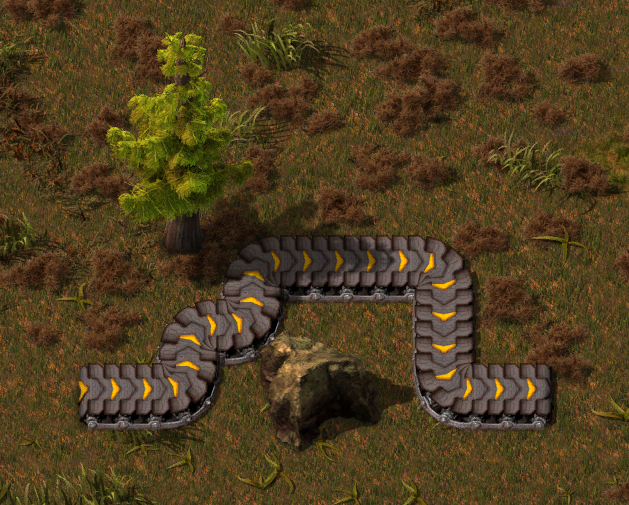
\includegraphics[width=0.8\textwidth]{img/factorio_complex-belt.png}
  \caption{Complex transport belt layout, avoiding a rock and a tree.}
  \label{fig:factorio_complex-belt}
\end{figure}

Finally, the compositions should also account for the machines taken up by the manufacturing.
Because in this domain we often use large numbers of machines, we use ``machine blocks'' to represent groups of machines performing the same recipe in parallel using common input and output flows.
These machine blocks integrate with logistics through these input and output flow locations.
Figure~\ref{fig:factorio_machine-block} depicts a block of four assembling machines in-game, all manufacturing iron gears from iron plates.

\begin{figure}[p]
  \centering
  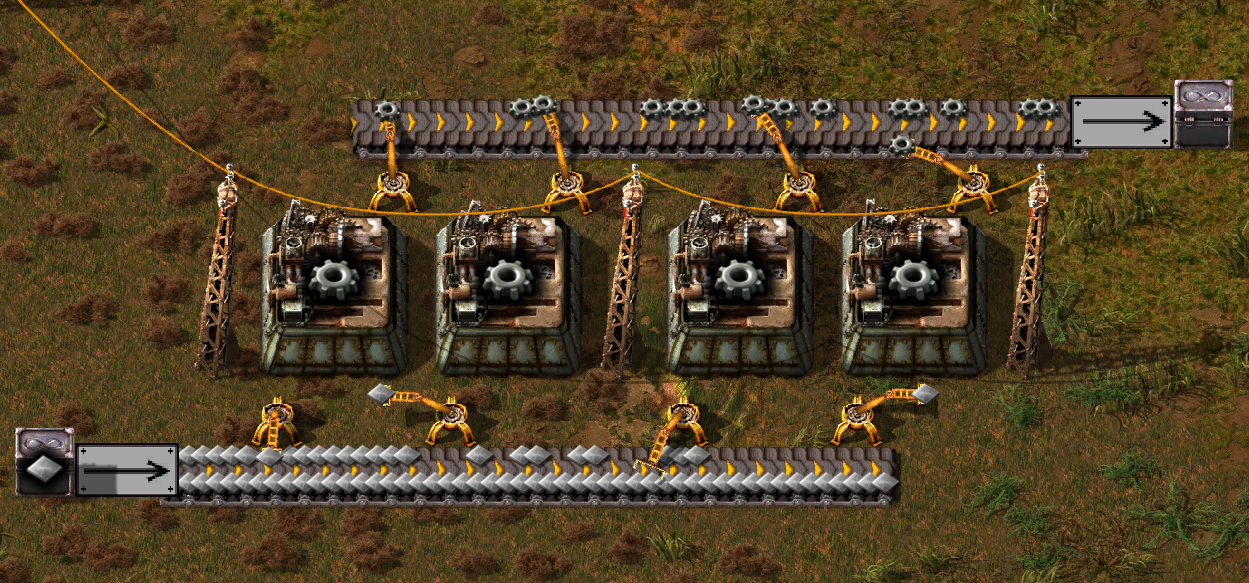
\includegraphics[width=\textwidth]{img/factorio_machine-block.png}
  \caption{Block of four assembling machines, all manufacturing iron gears from iron plates, with an input location on the left edge and output location on the right edge.}
  \label{fig:factorio_machine-block}
\end{figure}

We first define a domain with just item flows as resource atoms (see Section~\ref{sec:cases/factorio/item}) and primitive actions that represent logistics: splitting, merging and moving the flows (see Section~\ref{sec:cases/factorio/item-act}).
Then we extend this domain with machine blocks as further resource atoms (see Section~\ref{sec:cases/factorio/mach}), which allows us to represent manufacturing with a primitive action in the combined domain (see Section~\ref{sec:cases/factorio/manufacturing}).

As an application of the process models from this domain, we define how every valid composition can be turned into a sequence of instructions for its implementation in the game (see Section~\ref{sec:cases/factorio/instr}).
By mechanically following these instructions a player can implement the process.
Given a solution to the machine and logistics layout problems, an automated agent could also be made to mechanically follow these instructions.

This last part builds a text output (see Listing~\ref{lst:fourGears-instr} in Section~\ref{sec:cases/factorio/instr}) based on the given composition, so there is little we could gain by formalising it in Isabelle/HOL\@.
We instead implement it in Haskell on top of the formally verified code generated from the formalisation of this domain.

\subsection{Item Flows}
\label{sec:cases/factorio/item}

We start our formalisation of this domain by defining located flows of items.
For this we have to formalise locations, item types and rates of flow.

We only need locations to be uniquely identified, so that we know when two things are at the same location.
We choose to use string literals, rather than numeric identifiers, because they are more convenient when for example printed as part of the instructions.
The same reasoning applies when using string literals for action, item and machine labels in the rest of this section.
\begin{isadef}[Type synonym designating locations as string literals]{isa:factorio/loc}
  \isacomm{type-synonym}\ loc\ \isacharequal\ String.literal

\end{isadef}

We define item types simply by their label, such as an iron plate:
\begin{isadef}[Datatype for item types, with an example]{isa:factorio/item}
  \isacomm{datatype}\ item\ \isacharequal\ Item\ \isapars{\isafv{itemLabel}{\isacharcolon}\ String.literal}

\item
  \isacomm{definition}\ iron-plate\ \isacharequal\ Item\ \isaString{Iron\ Plate}

\end{isadef}

For rates of flow we use rational numbers (\isa{rat} in Isabelle/HOL).
They are sufficient to express rates and, compared to for instance the reals, their formalisation has a simple translation into executable code in the form of fractions.

Item flows simply combine the item type, rate of flow and location in one datatype:
\begin{isadef}[Datatype for flows of items]{isa:factorio/flow}
  \isacomm{datatype}\ flow\ \isacharequal\ Flow\ \isapars{\isafv{flowItem}{\isacharcolon}\ item}\ \isapars{\isafv{flowRate}{\isacharcolon}\ rat}\ \isapars{\isafv{flowLoc}{\isacharcolon}\ loc}

\end{isadef}

Because we will often be expressing item flows as individual resources, we define more convenient Isabelle notation for them:
\begin{isabelle}
\centering
  \isafv{item}\isalist{\isafv{rate}}\ \isanotation{at}\ \isafv{location}
\end{isabelle}
stands for:
\begin{isabelle}
\centering
  Res\ \isapars{Flow\ \isafv{item\ rate\ location}}
\end{isabelle}

\subsection{Logistics Actions}
\label{sec:cases/factorio/item-act}

We have five primitive actions representing logistics tools of the game for item flows (with first three shown in Figure~\ref{fig:factorio_move-split-merge}):
\begin{description}[style=nextline]
  \item[Moving a flow]
    Take a flow of given item type and rate from one location to another.
  \item[Splitting a flow]
    Split a flow into two flows of given rates.
    The rate the original flow must have is the sum of the given rates.
  \item[Merging flows]
    Take two flows of the same item at the same location and merge them into one.
  \item[Creating and empty flow]
    Create from nothing a flow of any item type at any location with zero rate.
  \item[Discarding an empty flow]
    Discard a flow of any item type at any location that has zero rate.
\end{description}

Before defining the actions themselves we specify the metadata they will carry.
In general, we use this data to support applications that inspect or consume compositions.
In this case, the application is the construction of a sequence of instructions for implementing the process.
Thus our metadata carries the information the user needs to implement each action.
We formalise the metadata in the same order as the inductive datatype \isa{flow{\isacharunderscore}meta} in Isabelle/HOL:
\begin{isadef}[Datatype for metadata of logistics actions]{isa:factorio/flow_meta}
  \isacomm{datatype}\ flow{\isacharunderscore}meta\ {\isacharequal}\isanewline
\ \ \isaindent{\isacharbar\ }Move\ \isapars{item}\ \isapars{rat}\ \isapars{loc}\ \isapars{loc}\isanewline
\ \ {\isacharbar}\ Split\ \isapars{item}\ \isapars{loc}\ \isapars{rat}\ \isapars{rat}\isanewline
\ \ {\isacharbar}\ Merge\ \isapars{item}\ \isapars{loc}\ \isapars{rat}\ \isapars{rat}\isanewline
\ \ {\isacharbar}\ Unit\ \isapars{item}\ \isapars{loc}\isanewline
\ \ {\isacharbar}\ Counit\ \isapars{item}\ \isapars{loc}

\end{isadef}

The processes in this domain then use item flows as linear atoms, no copyable atoms, string literals as labels and \isa{flow{\isacharunderscore}meta} as metadata.
We define the moving, merging and splitting of item flows as follows:
\begin{isadef}[Moving, splitting and merging flows of items]{isa:factorio/move_split_merge}
  \isacomm{definition}\ move\ {\isacharcolon}{\isacharcolon}\ {\isachardoublequoteopen}item\ {\isasymRightarrow}\ rat\ {\isasymRightarrow}\ loc\ {\isasymRightarrow}\ loc\isanewline
\isaindent{\isacomm{definition}\ move\ }{\isasymRightarrow}\ \isapars{flow,\ \isatv{c},\ String.literal,\ flow{\isacharunderscore}meta}\ process{\isachardoublequoteclose}\isanewline
\ \ \isaOcomm{where}\ {\isachardoublequoteopen}\isafv{move}\ \isabv{i\ r\ l\ k}\ {\isacharequal}\ Primitive\ {\isacharparenleft}\isabv{i}{\isacharbrackleft}\isabv{r}{\isacharbrackright}\ \isanotation{at}\ \isabv{l}{\isacharparenright}\ {\isacharparenleft}\isabv{i}{\isacharbrackleft}\isabv{r}{\isacharbrackright}\ \isanotation{at}\ \isabv{k}{\isacharparenright}\isanewline
\isaindent{\ \ \isaOcomm{where}{\isacharcolon}\ {\isachardoublequoteopen}\isafv{move}\ \isabv{i\ r\ l\ k}\ {\isacharequal}\ Primitive\ }\isaString{Move\ flow}\ {\isacharparenleft}Move\ \isabv{i\ r\ l\ k}{\isacharparenright}{\isachardoublequoteclose}%
\item
\isacomm{definition}\ split\ {\isacharcolon}{\isacharcolon}\ {\isachardoublequoteopen}item\ {\isasymRightarrow}\ loc\ {\isasymRightarrow}\ rat\ {\isasymRightarrow}\ rat\isanewline
\isaindent{\isacomm{definition}\ split\ }{\isasymRightarrow}\ \isapars{flow,\ \isatv{c},\ String.literal,\ flow{\isacharunderscore}meta}\ process{\isachardoublequoteclose}\isanewline
\ \ \isaOcomm{where}\ {\isachardoublequoteopen}\isafv{split}\ \isabv{i\ l\ r\ s}\ {\isacharequal}\ Primitive\ {\isacharparenleft}\isabv{i}{\isacharbrackleft}\isabv{r}{\isacharplus}\isabv{s}{\isacharbrackright}\ \isanotation{at}\ \isabv{l}{\isacharparenright}\ {\isacharparenleft}\isabv{i}{\isacharbrackleft}\isabv{r}{\isacharbrackright}\ \isanotation{at}\ \isabv{l}\ {\isasymodot}\ \isabv{i}{\isacharbrackleft}\isabv{s}{\isacharbrackright}\ \isanotation{at}\ \isabv{l}{\isacharparenright}\isanewline
\isaindent{\ \ \isaOcomm{where}\ {\isachardoublequoteopen}\isafv{split}\ \isabv{i\ l\ r\ s}\ {\isacharequal}\ Primitive\ }\isaString{Split\ flow}\ {\isacharparenleft}Split\ \isabv{i\ l\ r\ s}{\isacharparenright}{\isachardoublequoteclose}
\item
\isacomm{definition}\ merge\ {\isacharcolon}{\isacharcolon}\ {\isachardoublequoteopen}item\ {\isasymRightarrow}\ loc\ {\isasymRightarrow}\ rat\ {\isasymRightarrow}\ rat\isanewline
\isaindent{\isacomm{definition}\ merge\ }{\isasymRightarrow}\ \isapars{flow,\ \isatv{c},\ String.literal,\ flow{\isacharunderscore}meta}\ process{\isachardoublequoteclose}\isanewline
\ \ \isaOcomm{where}\ {\isachardoublequoteopen}\isafv{merge}\ \isabv{i\ l\ r\ s}\ {\isacharequal}\ Primitive\ {\isacharparenleft}\isabv{i}{\isacharbrackleft}\isabv{r}{\isacharbrackright}\ \isanotation{at}\ \isabv{l}\ {\isasymodot}\ \isabv{i}{\isacharbrackleft}\isabv{s}{\isacharbrackright}\ \isanotation{at}\ \isabv{l}{\isacharparenright}\ {\isacharparenleft}\isabv{i}{\isacharbrackleft}\isabv{r}{\isacharplus}\isabv{s}{\isacharbrackright}\ \isanotation{at}\ \isabv{l}{\isacharparenright}\isanewline
\isaindent{\ \ \isaOcomm{where}\ {\isachardoublequoteopen}\isafv{merge}\ \isabv{i\ l\ r\ s}\ {\isacharequal}\ Primitive\ }\isaString{Merge\ flows}\ {\isacharparenleft}Merge\ \isabv{i\ l\ r\ s}{\isacharparenright}{\isachardoublequoteclose}

\end{isadef}
\noindent
where, for instance, a \isa{merge\ \isafv{i\ l\ r\ s}} action takes two flows of the same item \isa{\isafv{i}} at the same location \isa{\isafv{l}} but with different rates \isa{\isafv{r}} and \isa{\isafv{s}}, and produces one with item and location unchanged but with summed rate.
The \isa{split} action does the opposite and the \isa{move} action changes only the location.
See Figure~\ref{fig:move-split-merge} for example diagrams of these actions and Figure~\ref{fig:factorio_move-split-merge} the in-game transport belt segments.

\begin{figure}[htbp]
  \centering
  \includesvg[scale=0.8]{img-gen/move-split-merge.svg}
  \caption{Process diagrams for example instances of \isa{move}, \isa{split} and \isa{merge}}
  \label{fig:move-split-merge}
\end{figure}

\begin{figure}[htbp]
  \centering
  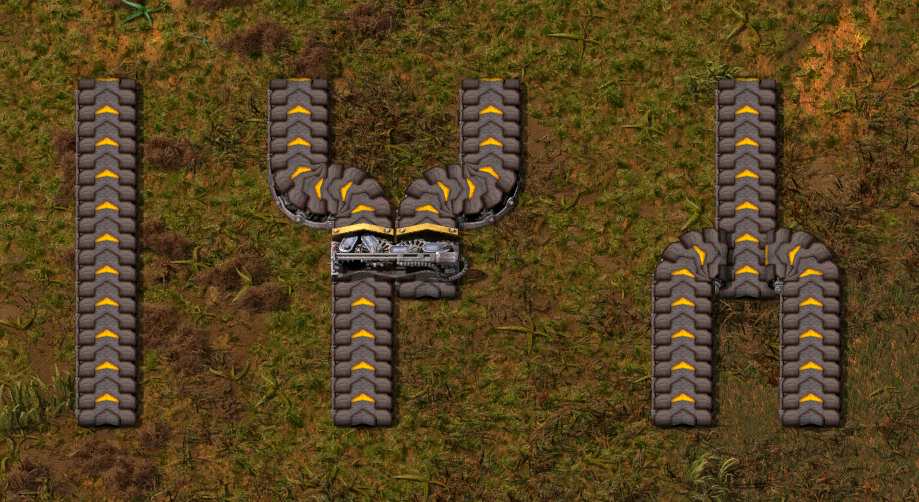
\includegraphics[width=\textwidth]{img/factorio_move-split-merge.png}
  \caption{Three transport belt segments representing the logistic actions \isa{move}, \isa{split} and \isa{merge} respectively.}
  \label{fig:factorio_move-split-merge}
\end{figure}

The remaining two actions represent our assumption that we can create and discard zero-rate flows for any item at any location.
We name these actions \isa{unit} and \isa{counit} and define them as follows, visualised with process diagrams in Figure~\ref{fig:unit-counit}:
\begin{isadef}[Creating and discarding zero-rate flows of items]{isa:factorio/unit_counit}
  \isacomm{definition}\isamarkupfalse%
\ unit\ {\isacharcolon}{\isacharcolon}\ {\isachardoublequoteopen}item\ {\isasymRightarrow}\ loc\ {\isasymRightarrow}\ \isapars{flow,\ \isatv{c},\ String.literal,\ flow{\isacharunderscore}meta}\ process{\isachardoublequoteclose}\isanewline
\ \ \isaOcomm{where}\ {\isachardoublequoteopen}\isafv{unit}\ \isabv{i\ l}\ {\isacharequal}\ Primitive\ Empty\ {\isacharparenleft}\isabv{i}{\isacharbrackleft}{\isadigit{0}}{\isacharbrackright}\ \isanotation{at}\ \isabv{l}{\isacharparenright}\ \isaString{Create\ zero\ flow}\ {\isacharparenleft}Unit\ \isabv{i\ l}{\isacharparenright}{\isachardoublequoteclose}
\item
\isacomm{definition}\isamarkupfalse%
\ counit\ {\isacharcolon}{\isacharcolon}\ {\isachardoublequoteopen}item\ {\isasymRightarrow}\ loc\ {\isasymRightarrow}\ \isapars{flow,\ \isatv{c},\ String.literal,\ flow{\isacharunderscore}meta}\ process{\isachardoublequoteclose}\isanewline
\ \ \isaOcomm{where}\ {\isachardoublequoteopen}\isafv{counit}\ \isabv{i\ l}\ {\isacharequal}\ Primitive\ {\isacharparenleft}\isabv{i}{\isacharbrackleft}{\isadigit{0}}{\isacharbrackright}\ \isanotation{at}\ \isabv{l}{\isacharparenright}\ Empty\ \isaString{Discard\ zero\ flow}\ {\isacharparenleft}Counit\ \isabv{i\ l}{\isacharparenright}{\isachardoublequoteclose}

\end{isadef}

\begin{figure}[htb]
  \centering
  \includesvg[scale=0.8]{img-gen/unit-counit.svg}
  \caption{Process diagrams for example instances of \isa{unit} and \isa{counit} actions}
  \label{fig:unit-counit}
\end{figure}

\subsection{Machine Blocks}
\label{sec:cases/factorio/mach}

Next we formalise machines and machine blocks, so that we can add them to the resource atoms and use them in manufacturing actions.
Machines are defined by their name, processing speed, base energy demand and running energy demand.
For instance, the electric furnace processes items at double of base speed, consumes $6\ kW$ of power while idle and an additional $180\ kW$ while running.
\begin{isadef}[Datatype for machines, with an example]{isa:factorio/machine}
  \isacomm{datatype}\ machine\ \isacharequal\isanewline
\ \ Machine\ \isapars{\isafv{machineLabel}{\isacharcolon}\ String.literal}\ \isapars{\isafv{machineSpeed}{\isacharcolon}\ rat}\isanewline
\isaindent{\ \ Machine\ }\isapars{\isafv{machineDrain}{\isacharcolon}\ nat}\ \isapars{\isafv{machineConsu}{\isacharcolon}\ nat}

\item
  \isacomm{definition}\ electric-furnace\ \isacharequal\ Machine\ \isaString{Electric\ Furnace}\ 2\ 6000\ 180000

\end{isadef}
\noindent
Note that the machine processing speed is a rational number to allow for machines taking more than base time (i.e.\ speed less than one).
The two energy demands, one when the machine is idle and one when it is running, are both natural numbers representing watts.

Machine blocks consist of the machine description, number of machines, input location and output location:
\pagebreak
\begin{isadef}[Datatype for blocks of machines working together]{isa:factorio/mach_block}
  \isacomm{datatype}\ mach-block\ \isacharequal\isanewline
\ \ MachBlock\ \isapars{\isafv{mblockMach}{\isacharcolon}\ machine}\ \isapars{\isafv{mblockCount}{\isacharcolon}\ nat}\isanewline
\isaindent{\ \ MachBlock\ }\isapars{\isafv{mblockIn}{\isacharcolon}\ loc}\ \isapars{\isafv{mblockOut}{\isacharcolon}\ loc}

\end{isadef}

As with item flows, we define more convenient Isabelle notation for machine blocks as individual resources:
\begin{isabelle}
\centering
  \isafv{mach}\isasymlangle\isafv{count}\isasymrangle\ \isanotation{at}\ \isafv{in-loc}\ \isanotation{\isasymrightarrow}\ \isafv{out-loc}
\end{isabelle}
stands for:
\begin{isabelle}
\centering
  Res\ \isapars{MachBlock\ \isafv{mach\ count\ in-loc\ out-loc}}
\end{isabelle}

\subsection{Manufacturing Action}
\label{sec:cases/factorio/manufacturing}

Manufacturing in our formalisation of this domain means using a block of machines to perform a recipe, converting one set of item flows into another.
Recipes are defined by two lists of item--count pairs (one for the inputs and one for the outputs), the base time required, the machine used and a name.
For instance, there is a recipe for crafting an iron gear from two iron plates, taking half a second and using a tier-one assembling machine.
\begin{isadef}[Datatype for manufacturing recipes, with an example]{isa:factorio/recipe}
  \isacomm{datatype}\isamarkupfalse%
\ recipe\ {\isacharequal}\isanewline
\ \ Recipe\ {\isachardoublequoteopen}\isapars{\isafv{recIn}{\isacharcolon}\ {\isacharparenleft}item\ {\isasymtimes}\ nat{\isacharparenright}\ list}{\isachardoublequoteclose}\ {\isachardoublequoteopen}\isapars{\isafv{recOut}{\isacharcolon}\ {\isacharparenleft}item\ {\isasymtimes}\ nat{\isacharparenright}\ list}{\isachardoublequoteclose}\isanewline
\isaindent{\ \ Recipe\ }\isapars{\isafv{recTime}{\isacharcolon}\ rat}\ \isapars{\isafv{recMach}{\isacharcolon}\ machine}\ \isapars{\isafv{recLab}{\isacharcolon}\ String{\isachardot}literal}

\item
  \isacomm{definition}\isamarkupfalse%
\ {\isachardoublequoteopen}craftGear\ {\isacharequal}\isanewline
\ \ Recipe\ {\isacharbrackleft}{\isacharparenleft}iron{\isacharunderscore}plate{\isacharcomma}\ {\isadigit{2}}{\isacharparenright}{\isacharbrackright}\ {\isacharbrackleft}{\isacharparenleft}iron{\isacharunderscore}gear{\isacharcomma}\ {\isadigit{1}}{\isacharparenright}{\isacharbrackright}\ {\isadigit{0}}{\isachardot}{\isadigit{5}}\ assembling{\isacharunderscore}machine{\isacharunderscore}{\isadigit{1}}\ \isaString{Craft\ Gear}

\end{isadef}

Performing a recipe with some number of machines in parallel requires flows of its inputs at one location and produces flows of its outputs at another location.
We define a function to help us construct these flows:
\begin{isadef}[Constructing a flow from recipe and machine information]{isa:factorio/stacksPerTimeAtSpeed}
  \isacomm{fun}\isamarkupfalse%
\ stacksPerTimeAtSpeed\ {\isacharcolon}{\isacharcolon}\ {\isachardoublequoteopen}rat\ {\isasymRightarrow}\ loc\ {\isasymRightarrow}\ nat\ {\isasymRightarrow}\ rat\ {\isasymRightarrow}\ item\ {\isasymtimes}\ nat\ {\isasymRightarrow}\ flow{\isachardoublequoteclose}\isanewline
\ \ \isaOcomm{where}\ {\isachardoublequoteopen}\isafv{stacksPerTimeAtSpeed}\ \isabv{t\ l\ n\ s}\ {\isacharparenleft}\isabv{i}{\isacharcomma}\isabv{c}{\isacharparenright}\ {\isacharequal}\ Flow\ \isabv{i}\ \isapars{\isabv{s}\ {\isacharasterisk}%
\ {\isacharparenleft}\isabv{n}{\isacharasterisk}\isabv{c}{\isacharparenright}\ {\isacharslash}\ \isabv{t}}\ \isabv{l}{\isachardoublequoteclose}

\end{isadef}
\noindent
which takes the recipe's time requirement \isa{\isabv{t}}, machine block location \isa{\isabv{l}}, number \isa{\isabv{n}} of parallel machines running the recipe, their processing speed \isa{\isabv{s}}, the item \isa{\isabv{i}} and its count \isa{\isabv{c}}, and constructs the corresponding item flow.
The last two arguments being taken as a pair is important to make this function suitable for mapping over the item--count lists with which recipes are defined.

The final piece of preparation is the metadata, which in this case collects the recipe, number of parallel instances, input location and output location:
\begin{isadef}[Datatype for metadata of the manufacturing action]{isa:factorio/manu_meta}
  \isacomm{datatype}\ manu{\isacharunderscore}meta\ {\isacharequal}\ Perform\ \isapars{recipe}\ \isapars{nat}\ \isapars{loc}\ \isapars{loc}

\end{isadef}

To express manufacturing actions, we move into a domain that combines both item flows and machine blocks.
This means that our processes now use as linear resource atoms the sum of those two types: \isa{flow\ \isacharplus\ mach{\isacharunderscore}block}.
Similarly, as metadata they use the sum of item flow and manufacturing metadata: \isa{flow{\isacharunderscore}meta\ \isacharplus\ manu{\isacharunderscore}meta}.
The two constructors of Isabelle's sum type, which inject a value from either summand into the sum type, are \isa{Inl\ \ty\ \isatv{a}\ \isasymRightarrow\ \isatv{a}\ \isacharplus\ \isatv{b}} and \isa{Inr\ \ty\ \isatv{b}\ \isasymRightarrow\ \isatv{a}\ \isacharplus\ \isatv{b}}.

We use a recipe, number of machines to use and two locations to define the manufacturing primitive action \isa{perform} as follows:
\begin{isadef}[Performing a recipe with a block of machines]{isa:factorio/perform}
  \isacomm{fun}\ perform\ {\isacharcolon}{\isacharcolon}\ {\isachardoublequoteopen}recipe\ {\isasymRightarrow}\ nat\ {\isasymRightarrow}\ loc\ {\isasymRightarrow}\ loc\isanewline
\isaindent{\isacomm{fun}\ perform\ {\isacharcolon}{\isacharcolon}\ }{\isasymRightarrow}\ {\isacharparenleft}flow\ {\isacharplus}\ mach{\isacharunderscore}block{\isacharcomma}\ \isatv{c},\isanewline
\isaindent{\isacomm{fun}\ perform\ {\isacharcolon}{\isacharcolon}\ {\isasymRightarrow}\ {\isacharparenleft}fl}String{\isachardot}literal{\isacharcomma}\ flow{\isacharunderscore}meta\ {\isacharplus}\ manu{\isacharunderscore}meta{\isacharparenright}\ process{\isachardoublequoteclose}\isanewline
\ \ \isaOcomm{where}\ {\isachardoublequoteopen}\isafv{perform}\ {\isacharparenleft}Recipe\ \isabv{ins\ outs\ time\ m\ name}{\isacharparenright}\ \isabv{n\ l1\ l2}\ {\isacharequal}\isanewline
\ \ Primitive\isanewline
\ \ \ \ {\isacharparenleft}\ Parallel\ {\isacharparenleft}map\ {\isacharparenleft}Res\ {\isasymcirc}\ Inl\ {\isasymcirc}\ stacksPerTimeAtSpeed\ \isabv{time}\ \isabv{l1}\ \isabv{n}\ {\isacharparenleft}machineSpeed\ \isabv{m}{\isacharparenright}{\isacharparenright}\isanewline
\isaindent{\ \ \ \ {\isacharparenleft}\ Parallel\ {\isacharparenleft}map\ }\isabv{ins}{\isacharparenright}\ {\isasymodot}\isanewline
\ \ \ \ \isaindent{\isacharparenleft}\ Res\ {\isacharparenleft}Inr\ {\isacharparenleft}MachBlock\ \isabv{m\ n\ l1\ l2}{\isacharparenright}{\isacharparenright}{\isacharparenright}\isanewline
\ \ \ \ {\isacharparenleft}\ Parallel\ {\isacharparenleft}map\ {\isacharparenleft}Res\ {\isasymcirc}\ Inl\ {\isasymcirc}\ stacksPerTimeAtSpeed\ \isabv{time\ l2\ n}\ {\isacharparenleft}machineSpeed\ \isabv{m}{\isacharparenright}{\isacharparenright}\isanewline
\isaindent{\ \ \ \ {\isacharparenleft}\ Parallel\ {\isacharparenleft}map\ }\isabv{outs}{\isacharparenright}{\isacharparenright}\isanewline
\ \ \ \ \isabv{name}\isanewline
\ \ \ \ {\isacharparenleft}\ Inr\ {\isacharparenleft}Perform\ {\isacharparenleft}Recipe\ \isabv{ins\ outs\ time\ m\ name}{\isacharparenright}\ \isabv{n\ l1\ l2}{\isacharparenright}{\isacharparenright}{\isachardoublequoteclose}

\end{isadef}
\noindent
where the input resource is a parallel combination of item flows (one for each input item of the recipe) along with a suitable block of machines.
The output resource is a parallel combination of only the item flows for the recipe's outputs.
The function \isa{machineSpeed} merely projects the second argument from the \isa{Machine} constructor, its processing speed.

Figure~\ref{fig:perform} shows an example diagram of the \isa{perform} action, using a recipe for making train cargo wagons.
It takes as input three item flows of the recipe ingredients (iron gears, iron plates, steel plates) arriving at the location named ``Source'' and the two assembling machines used to perform the recipe.
Those machines take inputs from ``Source'' and deposit their products at another location named ``Destination''.
See Figure~\ref{fig:fourGears} for further instances of this action.

\begin{figure}[htbp]
  \centering
  \includesvg[width=\textwidth]{img-gen/perform.svg}
  \caption{Process diagram for crafting cargo wagons on two machines in parallel.}
  \label{fig:perform}
\end{figure}

The machine block is consumed by this action to represent occupying those machines with continuous production.
This prevents us from using the same group of machines for two tasks at the same time.
The block's locations are set to match those where the input and output flows are generated, and its size is set to match the multiplier used to compute the flow rates.

With all the primitive actions set up we can proceed with constructing compositions.
In the following two sections we describe one such composition and how instructions are mechanically generated from such compositions.

From this point on we work in the combined domain, so we redefine our custom notation to use the appropriate injections.
The item flow notation \isa{\isafv{item}\isalist{\isafv{rate}}\ \isanotation{at}\ \isafv{location}} and the machine block notation \isa{\isafv{mach}\isasymlangle\isafv{count}\isasymrangle\ \isanotation{at}\ \isafv{in-loc}\ \isanotation{\isasymrightarrow}\ \isafv{out-loc}} now apply \isa{Inl} and \isa{Inr} respectively before constructing the resource atom.

Note that all processes from the item flow domain can be easily translated into the combined domain.
We just apply the left injection constructor \isa{Inl} to all linear resource atoms and metadata (leaving copyable atoms and labels unchanged) through the process map: \isa{map{\isacharunderscore}process\ Inl\ id\ id\ Inl}.
This map is defined automatically by Isabelle thanks to the BNF structure of resources (see Section~\ref{sec:res/bnf}).
See Section~\ref{sec:proc/transform} for a discussion of such systematic transformations of processes.

\subsection{Example Composition: Four Iron Gears}
\label{sec:cases/factorio/gears}

As an example composition we consider the process of turning iron ore into four iron gears per second.
This has two manufacturing steps: the iron ore must be smelted into plates and those then crafted into gears.
More precisely, considering the flow rates and locations, the process has four steps:
\begin{enumerate}
  \item Smelt iron ore into plates with $13$ furnaces in parallel.
  \item Split the resulting iron plates into two flows with rates $0.125$ and $8$.
  \item Move $8$ iron plates per second to the next location.
  \item Craft iron plates into gears with $4$ assembly machines in parallel.
\end{enumerate}

Our choice of targeting 100\% machine utilisation means that the furnaces produce more iron plates than we need, which could be made available to another process later on.
Alternatively, one could relax the utilisation requirement to require for $n$ machines utilisation of at least $\frac{n - 1}{n}$, meaning at most one machine from the group is not fully utilised.
Then the action of performing a recipe could be given a fractional number of parallel instances to meet any rational output flow rate.
We go with the 100\% requirement that sometimes yields a surplus, but our composition rules ensure that it is correctly accounted for and never lost (see Section~\ref{sec:proc/valid}).

The earlier four steps are reflected in the actual process composition, which is shown in Figure~\ref{fig:fourGears}:
Note that this composition is parameterised by the four involved locations, as they only have to be kept consistent between the individual actions.
In the second and third steps we translate logistics action, splitting and moving a flow respectively, into the combined domain using the process mapper.

\begin{figure}[htbp]
  \begin{subfigure}{\textwidth}
    \begin{isabelle}
      \isacomm{definition}\isamarkupfalse%
\ {\isachardoublequoteopen}\isafv{fourGears}\ \isabv{lIPlateIn\ lIPlateOut\ lGearIn\ lGearOut}\ {\isacharequal}\isanewline
\ \ \ \ {\isacharparenleft}\ perform\ smeltIronOre\ {\isadigit{1}}{\isadigit{3}}\ \isabv{lIPlateIn}\ \isabv{lIPlateOut}\ {\isasymparallel}\isanewline
\ \ \ \ \ \ Identity\ {\isacharparenleft}assembling{\isacharunderscore}machine{\isacharunderscore}{\isadigit{1}}{\isacharless}{\isadigit{4}}{\isachargreater}\isanotation{\ at\ }\isabv{lGearIn}\ {\isanotation{\isasymrightarrow}}\ \isabv{lGearOut}{\isacharparenright}{\isacharparenright}\ {\isacharsemicolon}{\isacharsemicolon}\isanewline
\ \ \ \ {\isacharparenleft}\ map{\isacharunderscore}process\ Inl\ id\ id\ Inl\ \isapars{split\ iron{\isacharunderscore}plate\ \isabv{lIPlateOut}\ {\isadigit{0}}{\isachardot}{\isadigit{1}}{\isadigit{2}}{\isadigit{5}}\ {\isadigit{8}}}\ {\isasymparallel}\isanewline
\ \ \ \ \ \ Identity\ {\isacharparenleft}assembling{\isacharunderscore}machine{\isacharunderscore}{\isadigit{1}}{\isacharless}{\isadigit{4}}{\isachargreater}\isanotation{\ at\ }\isabv{lGearIn}\ {\isanotation{\isasymrightarrow}}\ \isabv{lGearOut}{\isacharparenright}{\isacharparenright}\ {\isacharsemicolon}{\isacharsemicolon}\isanewline
\ \ \ \ {\isacharparenleft}\ Identity\ {\isacharparenleft}iron{\isacharunderscore}plate{\isacharbrackleft}{\isadigit{0}}{\isachardot}{\isadigit{1}}{\isadigit{2}}{\isadigit{5}}{\isacharbrackright}\isanotation{\ at\ }\isabv{lIPlateOut}{\isacharparenright}\ {\isasymparallel}\isanewline
\ \ \ \ \ \ map{\isacharunderscore}process\ Inl\ id\ id\ Inl\ \isapars{move\ iron{\isacharunderscore}plate\ {\isadigit{8}}\ \isabv{lIPlateOut}\ \isabv{lGearIn}}\ {\isasymparallel}\isanewline
\ \ \ \ \ \ Identity\ {\isacharparenleft}assembling{\isacharunderscore}machine{\isacharunderscore}{\isadigit{1}}{\isacharless}{\isadigit{4}}{\isachargreater}\isanotation{\ at\ }\isabv{lGearIn}\ {\isanotation{\isasymrightarrow}}\ \isabv{lGearOut}{\isacharparenright}{\isacharparenright}\ {\isacharsemicolon}{\isacharsemicolon}\isanewline
\ \ \ \ {\isacharparenleft}\ Identity\ {\isacharparenleft}iron{\isacharunderscore}plate{\isacharbrackleft}{\isadigit{0}}{\isachardot}{\isadigit{1}}{\isadigit{2}}{\isadigit{5}}{\isacharbrackright}\isanotation{\ at\ }\isabv{lIPlateOut}{\isacharparenright}\ {\isasymparallel}\isanewline
\ \ \ \ \ \ perform\ craftGear\ {\isadigit{4}}\ \isabv{lGearIn}\ \isabv{lGearOut}{\isacharparenright}{\isachardoublequoteclose}

    \end{isabelle}
    \caption{Definition of the process. We use \isa{\isacharsemicolon\isacharsemicolon} and \isa{\isasymparallel} as infix notation in Isabelle for sequential and parallel composition respectively.}
  \end{subfigure}
  \\~\\
  \begin{subfigure}{\textwidth}
    \centering
    \includesvg[width=\textwidth]{img/fourGears-cutup.svg}
    \caption{Process diagram.}
  \end{subfigure}
  \caption{Process definition and diagram for crafting iron gears from ore}
    \label{fig:fourGears}
\end{figure}

On top of the four core steps, the above composition also involves identity processes that ensure resources that are not being used in a given step are carried safely to the next.
One can find a pattern to these accommodations and define helper functions to more easily insert the identity processes, but we omit this to keep the example more direct.

Now we briefly discuss what implications there are from the validity of this composition, and more generally other compositions in this domain.
As discussed in Section~\ref{sec:proc/valid}, process composition validity in general requires that resources match on both sides of a connection.

Because two item flows are only equal if their rates are equal, we know that there is no bottleneck introduced from the connections made by the composition.
Then, because all of the manufacturing actions are set to run their machines at full capacity, we know the whole process will be running at 100\% utilisation.

Furthermore, item flows are also only equal if their locations are equal, which means that any change in item locations must come from primitive actions --- in our case either a movement or a manufacturing action.
Therefore these primitive actions describe all the required logistics connections.

Finally, the input and output of the composition tell us:
\begin{itemize}
  \item What items the process needs to keep working;
  \item What items it will produce;
  \item What kind of production capacity (i.e.\ machines) it requires to do so.
\end{itemize}
This information, along with the primitive actions contained in the composition, is all we need to generate instructions for implementing the composition as a factory in the game.
We discuss these instructions next, focusing on the process composition we introduced above.

\subsection{Generating User Instructions}
\label{sec:cases/factorio/instr}

We generate a sequence of instructions that can be mechanically carried out to build the factory.
In these we instruct the user on the placement and connection of the various machines.

Implementing our process compositions as factories in the game requires laying out each individual machine in the world and precisely routing the logistics connections.
In the absence of a fully automated solution for this problem, we rely on a human player to carry out the instructions.
The instructions may state that two locations should be connected, but they do not try to specify how exactly that connection should look in terms of coordinates.
However, if this layout is automated in the future, then our instructions could be adapted for an automated agent.

The instructions (see Listing~\ref{lst:fourGears-instr} for an example) are split into four parts:
\begin{itemize}
  \item Requirements, which are generated from the process input and state what item flows and machines need to be provided.
  \item Actions, which are generated from the primitive actions in the composition and describe how those should be implemented.
    For manufacturing this means describing the recipe and the machine block to use.
    For movement this means describing the item type, minimum required throughput, origin and destination.
  \item Effects, which are generated from the process output and state what item flows (and potentially unused machines) we get out of the process.
  \item Energy demand, which is calculated from the energy drain of machines consumed by the process.
    The fact that all used machines are fully utilised makes this calculation a simple sum.
\end{itemize}

\begin{lstlisting}[label=lst:fourGears-instr,caption=Instructions for the \isa{fourGears} composition,basicstyle=\small\ttfamily,columns=flexible,breaklines=true]
Process composition "fourGears":
Requirements:
 - Have Iron Ore arriving to iron-smelter-in at the rate of 65/8 per second
 - Have 13 of Electric Furnace taking inputs from iron-smelter-in and passing outputs to iron-smelter-out
 - Have 4 of Assembling Machine 1 taking inputs from gears-in and passing outputs to gears-out
Actions:
 - Set 13 of Electric Furnace to perform recipe "Smelt Iron Ore to Iron Plate" on inputs from iron-smelter-in and pushing outputs to iron-smelter-out
 - Split flow of Iron Plate located at iron-smelter-out from rate 65/8 per second into 1/8 per second and 8 per second
 - Move 8 per second of Iron Plate from iron-smelter-out to gears-in
 - Set 4 of Assembling Machine 1 to perform recipe "Craft Iron Plates into Iron Gear" on inputs from gears-in and pushing outputs to gears-out
Effects:
 - Have Iron Plate arriving to iron-smelter-out at the rate of 1/8 per second
 - Have Iron Gear arriving to gears-out at the rate of 4 per second
Energy demand: 2728000 W
\end{lstlisting}

The way we generate these instructions is the only part of our work on this domain that is outside of the proof assistant.
We use Haskell code automatically generated by Isabelle/HOL for all of the above definitions, including the \isa{fourGears} composition.
On top of this code we implement a number of functions for pretty-printing the data involved, such as printing the fully formal natural numbers as plain integers, and construct the actual instructions.
We construct individual instructions by taking the relevant part of the composition (e.g.\ its input or primitive actions) and expressing it in natural language.

We validated the above instructions for the \isa{fourGears} composition by carrying them out in-game, with the result shown in Figure~\ref{fig:factorio_four-gears}.
The resulting factory exhibits no bottlenecks between the machine blocks, just as validity of the composition predicts.
Furthermore, the production rates recorded by the simulation engine match those in the composition, and the recorded energy demand matches the one calculated from the consumed machines.
The only difficulty we encountered in following the instructions is implementing the precise item flow split ratio (in this case $1:64$) with the simple logistics tools made available (a $1:1$ splitter).

\begin{figure}[htbp]
  \centering
  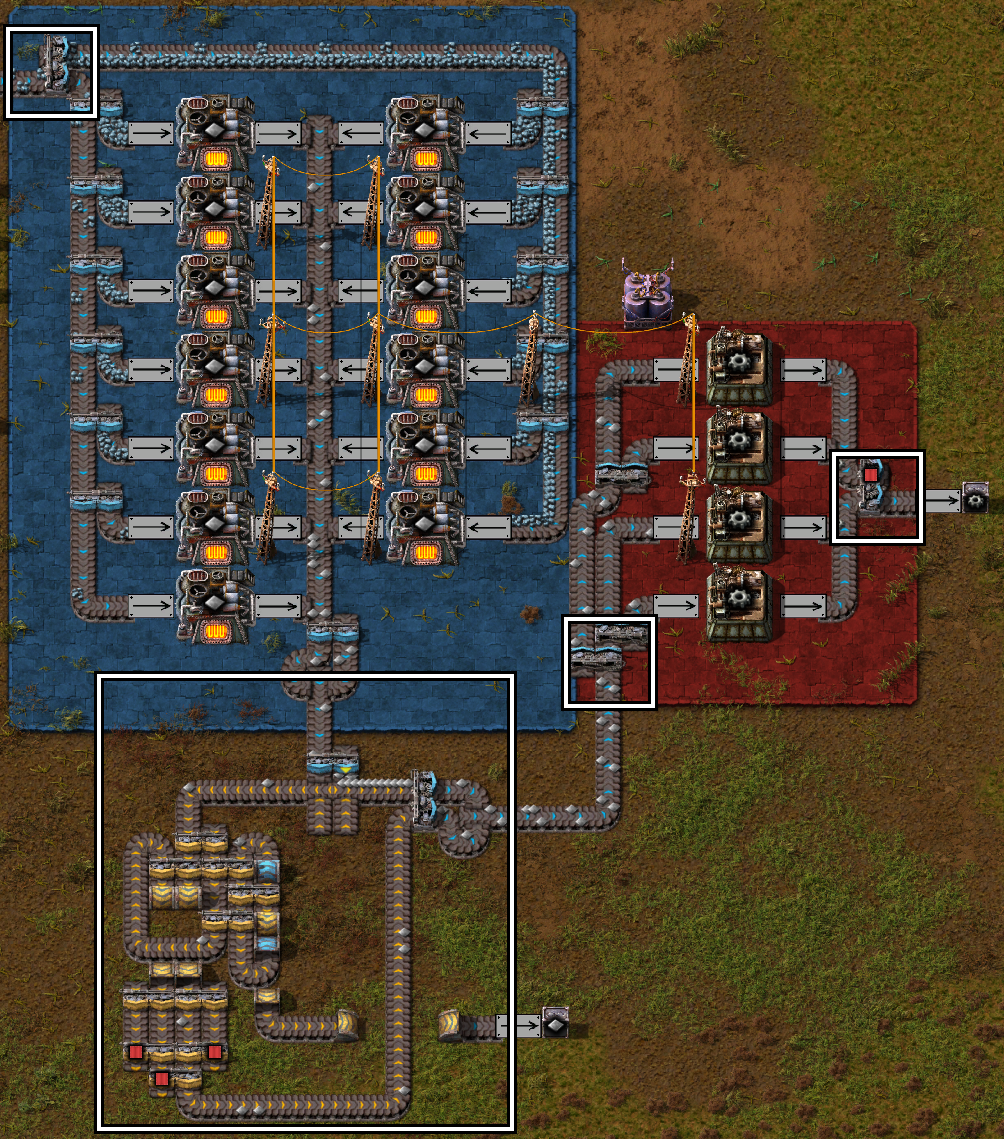
\includegraphics[width=\textwidth]{img/factorio_four-gears.png}
  \caption{In-game implementation of the \isa{fourGears} composition with the electric furnace block highlighted in blue and assembling machine block highlighted in red. The four named locations are highlighted with black-white squares. Bottom segment achieves the $1:64$ split of iron plates.}
  \label{fig:factorio_four-gears}
\end{figure}

\subsection{Possible Extensions}
\label{sec:cases/factorio/extensions}

While our formalisation of this domain is already non-trivial, there are still many aspects of Factorio that we do not model.
However, most of those could be modelled with our framework.
We note some here as possible future work extending this case study.

For instance, we currently only formalise solid manufacturing, while Factorio also involves fluids.
These have their own logistics system through the use of pipes, pumps and tanks.
They could be included in a way analogous to the item flows, while extending recipes and manufacturing actions to include them.

Another aspect we do not currently model in its entirety is fuel consumption.
We constrain ourselves only to machines that consume electricity, while the game also includes ones that consume solid or fluid fuels.
This could be included as a further input to performing a recipe, using the time taken, energy drain and energy value of a given fuel to compute how much is needed.

Beyond aspects of the game that we do not model, we could also improve the integration of our formalisation with the game.
At present, we manually encode the item types, machines and recipes that we use.
However, Factorio allows us to export the whole range of item types, machines and recipes from a running copy of the game as a JSON file.
We could load this data into Isabelle to make it all available to our formalisation with values guaranteed to be accurate.

\section{Conclusion}
\label{sec:cases/conc}

In this chapter we gave a number of case studies to demonstrate the main features of our framework.
We touch on a variety of domains: education, daily life and manufacturing.
The case studies we presented suggest some of the possible uses of our framework and the tools that could be based on it.

In the next chapter we conclude the thesis, tying together the thread running through it and giving a brief overview of potential future work.

\ifstandalone
\bibliographystyle{plainurl}
\bibliography{references}
\fi

\end{document}
